\documentclass{article}

\usepackage{enumerate}
\usepackage{amsthm}
\usepackage{amssymb}
\usepackage{bm}
\usepackage{geometry}
\usepackage{amsmath}
\usepackage{mathrsfs}
\geometry{
    a4paper,
    left=20mm,
    right=20mm,
    top=20mm,
    }
\usepackage{mathtools}
\mathtoolsset{showonlyrefs=true}
\newtheorem{thm}{Theorem}[subsection]

\newtheorem{Prob}{Theorem}[section]
\newtheorem{Prop}{Proposition}[section]
\newtheorem{Lem}{Lemma}[section]


\usepackage{xcolor}
\usepackage{graphicx}
\usepackage{hyperref}
\hypersetup{
    colorlinks=true,
    linkcolor=blue,
    filecolor=magenta,
    urlcolor=red,
}
\urlstyle{same}

\usepackage{pgfplots}
\usepackage{adjustbox}
% PGFPlots Version
\pgfplotsset{compat=newest}

%%% Declare %%%
\newcommand{\md}{\mathrm{d}}
\newcommand{\mR}{\mathbb{R}}
\newcommand{\trans}{\mathsf{T}}
\newcommand{\me}{\mathrm{e}}
\newcommand{\mi}{\mathrm{i}}
%%% Declare %%%

%%% custom %%%
\newcommand{\mM}{\mathcal{M}}
\newcommand{\mH}{\mathcal{H}}
\newcommand{\mA}{\mathcal{A}}
\newcommand{\mF}{\mathcal{F}}
\newcommand{\mX}{\mathcal{X}}
\newcommand{\mY}{\mathcal{Y}}
\newcommand{\mZ}{\mathcal{Z}}
\newcommand{\mO}{\mathcal{O}}
\newcommand{\mE}{\mathcal{E}}
% \newcommand{\mbE}{\mathbb{E}}
\newcommand{\mD}{\mathcal{D}}
\newcommand{\mS}{\mathcal{S}}
\newcommand{\mG}{\mathcal{G}}

\DeclareMathOperator*{\argmin}{argmin}
\DeclareMathOperator*{\diag}{diag}
\DeclareMathOperator*{\tr}{Tr}
\DeclareMathOperator*{\mbE}{\mathbb{E}}
\DeclareMathOperator{\sech}{sech}

\DeclareMathOperator{\skiploss}{\mathcal{L}^{\mathrm{skip}}}
\DeclareMathOperator{\weightedloss}{\mathcal{L}^{\mathrm{weighted}}}

%%$ custom %%%
\usepackage[all]{xy}
\usepackage{subcaption}
% \usepackage{footmisc}
%%% document info %%%
\title{Latent Assimilation with Implicit Neural Representations for Unknown Dynamics}
\author{Zhuoyuan Li}
\date{\href{mailto:zy.li@stu.pku.edu.cn}{zy.li@stu.pku.edu.cn}}
%%%


\begin{document}
\maketitle
\section{Introduction}
Data assimilation (DA) has increasingly become an indispensable tool across a multitude of disciplines, including weather forecasting, climate modeling, oceanography, ecology, and even economics. The core idea of data assimilation is the integration of the information derived from disparate sources, such as in situ observations and satellites data, with physical models that describe the underlying dynamics of the system. The objective of DA is to obtain the best estimate of the system states, in line with both observation data and physical models, while considering their inherent uncertainties.

From a mathematical standpoint, DA algorithms are efficient and practical solutions to a particular inverse problem
\[\bm y=\mF(\bm x)+\bm\eta.\]
Here, $\bm x$ signifies system states of interest, with $\bm y$ representing observation data, $\mF$ being the observational operator, and $\bm\eta$ standing for an additive noise. For instance, within the context of modern numerical weather prediction (NWP), $\bm x$ may consist of all atmospheric variables at a single or multiple time steps, with DA framworks employed to determine optimal initial conditions. Such problem is often addressed by Bayesian point of view, where the posterior probability $p(\bm x\mid\bm y)$ is evaluated as
\[p(\bm x\mid\bm y)=\frac{p(\bm y\mid\bm x)p(\bm y)}{p(\bm y)}\propto p(\bm y\mid\bm x)p(\bm x)\]
and subsequently maximized. The likelihood term $p(\bm y\mid\bm x)$ and the prior term $p(\bm x)$ correspond to the observation model and the system's underlying dynamic model, respectively. Hence, maximizing the posterior probability effectively equates to adjusting the state $\bm x$ to best align with both the observation data and the physical models.

Current DA frameworks largely draw upon either three/four-dimensional variational (3/4d-Var) methods or Kalman filter methods. The former employs a variational optimization-based approach that assimilates data over a fixed time window, while the latter utilizes a recursive estimation algorithm that operates sequentially in real-time. Nonetheless, both these are faced with challenges linked to system dimensionality. As the dimension of the state $\bm x$ increases dramatically in practical scenarios, the optimization processes for variational methods become inevitably expensive, and the direct storage and updates required for the covariance matrices in Kalman filters turn infeasible. Although the ensemble methods can alleviate these issues to some extent, they confine the assimilated states within a low-dimensional subspace, potentially harming the overall performance. Another significant limitation is the restricted handling of nonlinearity. Consequently, the development of advanced DA frameworks capable of efficiently managing high-dimensional systems is an area of considerable interest.
\subsection{Leveraging Reduced-Order-Models for Latent Assimilation}
One promising approach to address the issues related to high-dimensionality is the use of Reduced-Order-Models (ROMs) as approximations for the system. At the core of these methods is the assumption that a low-dimensional submanifold $\mX'$ exists within the system state space $\mX$, where all system states $\bm x$ reside. By defining a suitable parameterization $\{\bm x_{\bm z}\}_{\bm z\in\mZ}$ of $\mX'$, a one-to-one correspondence between the parameterized (or latent) space $\mZ$ and the submanifold $\mX'$ can be established. With the explicit derivation of the dynamics on $\mZ$ and the bijective relation between $\mZ$ and $\mX'$, the DA algorithms can be transitioned to operate within the latent space. We refer to such DA process within the latent space as latent assimilation (LA). Given that the dimension of the latent space typically satisfies $\dim\mZ\ll\dim\mX'$, both the storage and computational cost of LA are reduced in comparison with the original DA.

Classical ROMs are usually linear which make use of proper orthogonal decomposition (POD) method or wavelet decomposition to extract the system's dominant modes a collection of history snapshots. Under these circumstances, $\mX'$ is defined as the optimal low-dimensional subspace of $\mX$, spanned by the dominant modes, which minimizes the reconstruction error. The corresponding parameterizations $\bm z\in\mZ$ for each state $\bm x$ are the projection coefficient vectors onto each mode. These methods are not only straightforward to implement, but also offer simple linear bijective mappings between $\mZ$ and $\mX'$, which simplify the derivation of the latent dynamics on $\mZ$. However, the reconstruction accuracy is heavily dependent on the number of dominant modes, and as the system becomes more complicate, much more dominate modes are required to reconstruct the small-scale structures, which decreases the effectiveness of reduction of dimensionality.

\subsection{Related works and contributions}
In recent years, the explosive growth of Machine Learning (ML) and, specifically, Deep Learning (DL) methods has made remarkable strides in a wide array of disciplines, including image restoration, natural language processing, and generative modeling. The application of DL in solving complex physical problems, such as solving differential equations \cite{PINNs,DeepRitz,DeepGalerkin}, discovering underlying physical laws \cite{PDENet2.0,SINDy,AI-Feyman}, and simulating spatio-temporal dynamics \cite{DeepONet,FNO}, has attracted significant attention and achieved promising results.

In the realm of atmospheric sciences, DL-based approaches have great success in handling a variety of tasks, including weather forecasting, post-processing as well as data assimilation. The positive trend has dispelled doubts \cite{Schultz2021CanDL} about DL's capability to manage intricate dynamics, with notable models like FourCastNet \cite{FourCastNet}, followed by Pangu-Weather \cite{Pangu}, GraphCast \cite{GraphCast} and FengWu \cite{FengWu} focusing on weather forecasting tasks.

The idea of ROMs, which utilize dimensionality reduction methods to represent high-dimensional space with lower-dimensional ones, has been well developed in the field of DL, and some early works \cite{Peyron2021LAwithAE,LatentspaceDA-RNN,ROM-DA,GeneralizedLA} have been proposed in the context of data assimilation. By transforming system state variables into lower-dimensional latent codes using encoder-decoder network structures, surrogate models for latent dynamics are trained simultaneously. However, existing ROMs based on fully-connected networks, Recurrent Neural Networks (RNNs), and Long Short-Term Memory (LSTM) networks face challenges regarding scalability, computational efficiency, and applicability to fixed-grid input data. Table \ref{tab:related_works} summarizes the comparative strengths and weaknesses of these methods.
% Establishing ROMs by using neural networks is not a new idea. Note that ROMs may have multiple meanings such as network model compression and knowledge distillation in the context of DL, and we have to clarify that the ROMs we are talking about throughout the work are dimensionality reduction methods, which is to represent vectors lying in a high-dimensional space by a low-dimensional ones. We borrow the terminology from the community of DL, where the mapping from the high-dimensional system state space to the low-dimensional latent space is called the encoder, and the mapping in the reversed direction is called the decoder.
% To address DA problems with ROMs implemented via DL, researchers have proposed various encoder-decoder network structures to transform the system state variables $\bm X\in\mX$ into latent codes $\bm z\in \mZ$ of lower dimension. Then another network is trained to play an role as a surrogate model for the latent dynamics. Both the encoder-decoder network and the latent dynamics network are trained with a number of data sampled from the original dynamical system. 

The work of \cite{Peyron2021LAwithAE} selects trivial fully-connected deep neural networks for both the encoder and the decoder, and the latent dynamics is approximated via ReZero\cite{bachlechner2021rezero} as a variant of ResNet\cite{He2015ResNet} to enhance the stability. In spite of the unawareness of explicit dynamics, the performance is comparable even with classical DA with known dynamics. Besides, the forward propagation is accelerated by latent embedding. Unfortunately, the fully-connected architecture can hardly be applied to multi-dimensional cases since the storage and training for the huge number of network parameters are unaffordable. Recurrent Neural Networks (RNNs) can serve as an alternative way for evolving latent dynamics as proposed in \cite{LatentspaceDA-RNN}, which merges the encoder-decoder structure into RNNs. The training of RNNs takes the advantage of Reservoir Computing (RC) \cite{ReservoirComputing} to make the forward propagation faster, but as suggested in \cite{Arcomano2020MLGAFM,LatentspaceDA-RNN}, the RC approaches are more suitable for short-term prediction tasks. Meanwhile, creating patches when scaling to high-dimensional problems can probably result in disagreement between neighborhoods. To effectively capture long-term dependencies in sequencial data, Long Short-Term Memory (LSTM) networks have been employed in \cite{ROM-DA,GeneralizedLA}, but they face the same issues as those of \cite{Peyron2021LAwithAE} that the model is not scalable to high-dimensional problems. In addition, the LSTM-based models slowen the forward propagation process, which needs to be called frequently in assimilation algorithms. Finally, all the the architectures mentioned above require the input data lying on certain fixed grids unless interpolations probably resulting in additional errors are applied.
\renewcommand{\arraystretch}{1.2}
\begin{table}
	\centering
	\begin{tabular}{c|c|c|c|c|c}
		\hline
		method                            & encoder-decoder  & latent dynamics & scalability & efficiency & mesh-free \\
		\hline
		ETKF-Q-L\cite{Peyron2021LAwithAE} & fully-connected  & ReZero          & low         & high       & no        \\
		RNN-ETKF\cite{LatentspaceDA-RNN}  & RNN              & RC              & medium      & high       & no        \\
		NIROM-DA\cite{ROM-DA}             & POD/PCA          & LSTM            & low         & medium     & no        \\
		GLA \cite{GeneralizedLA}          & POD/PCA + Conv1d & LSTM            & low         & medium     & no        \\
		LAINR (ours)                      & INR              & Neural ODE      & high        & medium     & yes       \\
		\hline
	\end{tabular}
	\caption{Comparison of different methods for latent assimilation. The method names are borrowed from the original papers.}
	\label{tab:related_works}
\end{table}
\renewcommand{\arraystretch}{1.0}

In this work, we present the Latent Assimilation with Implicit Neural Representations (LAINR) framework, which is to our best knowledge, the first mesh-free DA method designed for multi-dimensional unknown dynamics. By proposing the LAINR framework, we aim to make a meaningful contribution to the ongoing exploration of DL and ML techniques in data assimilation and atmospheric sciences. The primary contributions of our work are:
\begin{itemize}
	\item We introduce a mesh-free encoder-decoder structure for LA, employing Implicit Neural Representations (INR) to approximate system states. This structure is scalable and applicable to multi-dimensional problems.
	\item We validate the effectiveness of our proposed method through experiments on the shallow water equations, demonstrating the high accuracy, stability, and robustness of the LAINR framework.
\end{itemize}
\section{Latent-space embedding and dynamics learning}
Latent Assimilation (LA) is essentially a form of Data Assimilation (DA) methodology where the model space is characterized by a latent space, denoted by $\mZ$, rather than the physical state space $\mX$. Similar to conventional DA methods, the construction of an effective LA model necessitates the specification of the forward propagation on the latent space $\mZ$ and the associated observation operator that bridges $\mZ$ to the observational space $\mY$ (Figure \ref{fig:comp-DA-and-LA}). Additionally, uncertainty considerations brought by noise must be incorporated into these mappings. Our work aims to explore the choice of latent-space embeddings and surrogate models for latent dynamics under this LA context.
\begin{figure}[!h]
	\centering
	\begin{subfigure}{.45\textwidth}
		\[
			\xymatrix{
				\cdots\ar[r]^\mM&\mX\ar[r]^{\mM}\ar[d]_{\mH}&\mX\ar[d]^{\mH}\ar[r]^\mM&\cdots\\
				&\mY&\mY&
			}
		\]
		\caption{classical DA framework}
	\end{subfigure}
	\hfill
	\begin{subfigure}{.45\textwidth}
		\[
			\xymatrix{
			\cdots\ar[r]^\mG&\mZ\ar[r]^{\mG}\ar@/^1ex/[d]^{\mD}&\mZ\ar@/^1ex/[d]^{\mD}\ar[r]^\mG&\cdots\\
			\cdots\ar[r]^\mM&\mX\ar@/^1ex/[u]^{\mE}\ar[r]^{\mM}\ar[d]_{\mH}&\mX\ar@/^1ex/[u]^{\mE}\ar[d]^{\mH}\ar[r]^\mM&\cdots\\
			&\mY&\mY&
			}
		\]
		\caption{latent assimilation (LA) framework}
	\end{subfigure}
	\caption{Comparison between classical DA and LA frameworks.}
	\label{fig:comp-DA-and-LA}
\end{figure}

Our work operates under the assumption that a low-dimensional parameterization exists for the high-dimensional system states, thus, we present detailed discussions about the latent embedding and learning of latent dynamics. Let $\mX=\mR^n$ and $\mZ=\mR^m$ denote the system state space and the latent space, respectively, where $n$ is considerably larger than $m$. The goal of latent embedding is to determine a pair of encoder $\mE:\mX'\to\mZ$ and decoder $\mD:\mZ\to\mX'$ that are essentially inverse mappings between the low-dimensional submanifold $\mX'$ that encapsulates all possible system states, and the latent space $\mZ$.

Let's assume that the system state variable we aim to assimilate is $\bm u:\mR^d\to\mR^c$, where $d$ signifies the inherent dimension of the system (usually $2$ or $3$), and $c$ refers to the number of features of interest (such as horizontal wind, temperature, humidity, and so forth). Given a fixed sampling grid $G\subseteq\mR^d$, we explore various approaches to build a reduced-order model for the system state $\bm x=\{\bm u(\bm p)\}_{\bm p\in G}\in\mR^{|G|\times c}=\mR^n$. Table \ref{tab:comp_latent_embedding} offers a summary of distinct choices for the encoder $\mE$ and the decoder $\mD$.

\renewcommand{\arraystretch}{1.5}
\begin{table}[!h]
	\centering
	\begin{tabular}{c|c|c|c}
		\hline
		method & encoder $\mE$                                                             & decoder $\mD$                                            & error to be minimized                                                             \\
		\hline
		POD    & $\bm x\mapsto A^\trans\bm x$                                              & $\bm z\mapsto A\bm z$                                    & $\left\|\left(I_n-A^\trans A\right)\bm X\right\|_F^2$ subject to $A^\trans A=I_m$ \\
		AE     & $\bm x\mapsto f_\theta(\bm x)$                                            & $\bm z\mapsto g_\varphi(\bm z)$                          & $\mathcal{L}(\bm x,g_\varphi(f_\theta(\bm x)))$                                   \\
		INR    & $\bm x\mapsto\argmin_{\bm z}\|I(\cdot;\bm z,\bm\varphi)-\bm u\|_{\mu(G)}$ & $\bm z\mapsto\{I(\bm p;\bm z,\bm\varphi)\}_{\bm p\in G}$ & $\|I(\cdot;\bm z,\bm\varphi)-\bm u\|_{L^p(\mu)}$                                  \\
		\hline
	\end{tabular}
	\caption{Comparison of different methods for latent embedding.}
	\label{tab:comp_latent_embedding}
\end{table}
\renewcommand{\arraystretch}{1.0}

\subsection{Classical linear ROMs}\label{sec:linear-encoders}
In the domain of classical ROMs, we typically encounter linear methods like Proper Orthogonal Decomposition (POD) or wavelet decomposition that provide a low-dimensional representation of the system. We introduce such linear ROMs by take the method of POD as an example. POD aims to identify a set of orthogonal basis vectors ${\bm\phi_j}_{j=1}^m\subseteq\mR^n$, known as dominant modes, that minimize the projection error on expectation. Formally, given a series of historical ground truths or assimilated data ${\bm x_k}_{k=1}^K$, the objective of POD is to determine the dominant modes such that
\[\{\bm\phi_j\}_{j=1}^m=\argmin_{\bm\phi_j}\mbE_{\bm x\sim\mathscr{D}}\|\bm x-\widehat{\bm x}\|^2,\]
where $\mathscr{D}$ denotes the distribution of system states $\bm x\in\mX$, and $\widehat{\bm x}$ is the projection of $\bm x$ onto the linear subspace spanned by $\{\bm\phi_j\}_{j=1}^m$. $m$ is the number of dominant modes usually fixed in advance. Since the explicit form of $\mathscr{D}$ is often difficult to derive in practice, the expectation is approximated empirically, i.e.,
\[\{\bm\phi_j\}_{j=1}^m=\argmin_{\bm\phi_j}\frac1K\sum_{k=1}^K\|\bm x_k-\widehat{\bm x_k}\|^2.\]
It is worth noting that the projections $\widehat{\bm x_k}$ can be explicitly expressed as
\[\widehat{\bm x_k}=\sum_{j=1}^m\langle\bm x_k,\bm\phi_j\rangle\bm\phi_j,\]
where $\langle\cdot,\cdot\rangle$ denotes the inner product in $\mX=\mR^n$. Consequently, the optimization problem can be rewritten in the form
\[A:=(\bm\phi_1,\cdots,\bm\phi_m)^\trans=\argmin_A\frac1K\sum_{k=1}^K\left\|\bm x_k-A^\trans A\bm x_k\right\|^2=\argmin_A\sum_{k=1}^K\left\|\left(I_n-A^\trans A\right)\bm x_k\right\|^2\textrm{ s.t. }AA^\trans =I_m,\]
which can be solved by the singular value decomposition (SVD) of the empirical covariance matrix $\bm X\bm X^\trans$. More specifically, the target function is minimized when the rows of $A$ are the first $m$ left singular vectors of the matrix $\bm X=(\bm x_1,\cdots,\bm x_K)\in\mR^{n\times K}$ (See Prop. \ref{prop:pod_optimality} for a detailed proof). Such operations are often referred to as the Principal Component Analysis (PCA).

Overall, the key benefit of POD in this context is that the dominant modes ${\bm\phi_j}{j=1}^m$ can be obtained directly without training, offering an efficient and direct way to generate a linear reduced-order model, and the encoder-decoder mappings are defined as $\mE^{\textrm{POD}}:\bm x\mapsto A\bm x$ and $\mD^{\textrm{POD}}:\bm z\mapsto A^\trans\bm z$, respectively.

\subsection{Autoencoders: non-linear representations and limitations}
Autoencoders, as a common neural network architecture in deep learning, introduce a non-linear dimensionality reduction approach that expands upon the concept of latent space. With an encoder $\mE^{\textrm{AE}}=f_\theta$ and a decoder $\mD^{\textrm{AE}}=g_\varphi$, this architecture can skillfully navigate high-dimensional input data, extracting a lower-dimensional latent space representation in the process. The encoder progressively decreases the data dimension with its multi-layered structure. By mirroring the encoder's architecture, the decoder takes the encoded representations and then reconstruct the original input data.

An autoencoder's objective is to minimize the empirical reconstruction error by employing a loss function to measure the divergence between the input and reconstructed data. The optimization process for
\[\theta,\varphi=\argmin_{\theta,\varphi}\sum_{k=1}^K\mathcal{L}(\bm x_k,g_\varphi(f_\theta(\bm x_k)))\]
promotes the learning of compressed meaningful data representation.

Compared with POD, autoencoders are capable of capturing non-linear relationships in the data, which is crucial for the latent dynamics learning since it introduces the possibility of simplifying a complex dynamical system in the physical space into a more manageable latent dynamics. Moreover, autoencoders bring flexibility due to their various structures. For instance, autoencoders can be designed to focus on local correlations with the help of convolutional networks. With structures like Recurrent Neural Networks (RNN), such as LSTM \cite{LSTM} and GRU \cite{GRU}, they can even process sequential data naturally.

Despite the promise of autoencoders, there still exist lots of limitations.
Unlike linear ROMs like PCA, they do not ensure an optimal representation even in the empirical sense since the minimizer is not guaranteed to be obtained. Besides, the training process is considerably more time-consuming as the selections of network architectures and hyperparameters need to be determined carefully. Furthermore, autoencoders may face scalability challenges when dealing with high-dimensional problems as the number of grid points will increase exponentially with respect to the state dimension and resolutions. Such complexity could lead to cumbersome and resource-intensive training processes, which is where implicit neural representations (INRs) as our main focus may offer a viable alternative. The scalability and reduced complexity of INRs render them more conducive to high-dimensional problems, ensuring efficient training and implementation.
\subsection{Implicit neural representations}
Implicit Neural Representations (INRs) adopt a distinct approach to data modeling that deviates from traditional grid-vased or mesh-mased methods such as the autoencoder described earlier. Rather than operating on state features on discrete positions, INRs ingest coordinate information and model signals or fields as continuous mappings, which provides a substantial advantage when working with continuous underlying signals or fields that are only available at discrete grid points or mesh intersections.

The core idea of INR is to use a parameterized neural network $I(\cdot;\bm z,\bm\varphi)$ to approximate the system state of interest $\bm u:\mX\to\mR^c$. The network aims to minimize the disparity between $I(\cdot;\bm z,\bm\varphi)$ and $\bm u$, measured with an appropriatem measure $\mu$ defined on a fixed grid $G$. The parameter $\bm\varphi$ captures consistent field properties and thus remains invariant across the dataset. On the other hand, the latent vector $\bm z$ containing the physical features shifts with different time steps. As an example, one may choose the $L^2$ norm with $\mu$ being a sum of Dirac delta functions $\mu=|G|^{-1}\sum_{\bm p\in G}\delta_{\bm p}$, which results in a minimization problem for
\[\|I(\cdot;\bm z,\bm\varphi)-\bm u\|_{L^2(\mu)}=\frac{1}{|G|}\sum_{\bm p\in G}|I(\bm p;\bm z,\bm\varphi)-\bm u(\bm p)|^2.\]
INRs present multiple advantages. Their independence of the explicit form of underlying grids or spatial resolutions promotes the flexibility. Meanwhile, similar to autoencoders, the non-linearity inherent to neural networks enables them to capture the intricate non-linear correlations, which outperforms classical linear ROMs like POD. Such advantages have been leveraged firstly in the field of shape modeling which have demostrate the superiority over grid-based and mesh-based archtectures \cite{chen2019learning,park2019deepsdf}. Since then, INRs have been applied to a variety of fields including image processing \cite{sitzmann2019siren,Bemana2020xfields,dupont2022coinpp} and spatio-temporal dynamics \cite{Jiang2020MeshfreeFlowNet,chen2023crom,yin2023dino}.

In the context of INRs, the encoder involves solving an optimization problem
\[\mE^{\textrm{INR}}\left(\left\{\bm u(\bm p)\right\}_{\bm p\in G}\right)=\bm z=\argmin_{\bm z}\|I(\cdot;\bm z,\bm\varphi)-\bm u\|_{L^p(\mu)}.\]
The high cost for the optimization problem is a major concern in most INR-based methodologies, but as explained later, the LAINR framework remains efficient since the optimization needs to be executed only at the initialization stage. Conversely, given the latent representation $\bm z$, the system state is directly recovered by $I(\cdot;\bm z,\bm\varphi)$ as a continuous signal or field.
\subsection{Evolution of latent dynamics}
Establishing a suitable surrogate model for the evolution of latent dynamics forms another crucial part for the LA framework, which not only addresses the non-linearity of the system dynamics but also integrates the auto-regressive property for the evolution of latent dynamics, regardless of whether or not the explicit form of the physical dynamics are provided. For simplicity, we assume that the latent dynamics are time-invariant and thus approximated by a parameterized surrogate model $\mG_{\bm\psi}$ such that the differences between $\bm z_{k+1}$ and $\mG_{\bm\psi}(\bm z_{k})$ are minimized.

The choices for the structure of $\mG_{\bm\psi}$ can be far more diverse, which strongly depends on the specific characteristics of the system state's temporal dynamics. For instance, Long Short-Term Memory (LSTM)\cite{LSTM} units and Gated Recurrent Units (GRUs)\cite{GRU} are specially designed for sequential data, whose structure enable the network to remenber or forget previous states based on the context. Another kinds of modelling the sequential data are motivated by the classical numerical integrators for differential equations. Deep Residual Nets (ResNets)\cite{He2015ResNet} have been promoted to accelerate the training process of deep networks at first, which add skip connections to mitigate the problem of vanishing and exploding gradients. However, ResNet models are essentially a discretization of the continuous-time system and are subject to issues related to step size and temporal resolution. On the contrary, Neural ODEs, introduced by \cite{chen2018NeuralODE,chen2021eventfn}, consider a neural network as a continuous-time dynamical system. In the current work, we do not dive deeply into the optimal structure of the surrogate model, but the experimental performances suggest that using a network implemented by NeuralODE \cite{chen2018NeuralODE,chen2021eventfn} have shown superiority over ResNet. Furthermore, compared with ResNet, NeuralODE is more suitable for comtinuous-time dynamical system and more flexible as it allows variable lengths of time steps.
\section{Latent assimilation framework}
Classical data assimilation methods require observed data $\{\bm y_k\}_k$, observation operators $\{\mH_k\}_k$, forward propagation operators $\{\mM_k\}_k$ describing the system dynamics as well as a background estimate $\bm x_0$ for start-up. Meanwhile, the noise modeling is indispensable to help track the evolution of the error and then derive the assimilated state. Once the encoder-decoder mappings $\mE$, $\mD$ and the surrogate model $\mG$ have been obtained via either deterministic algorithm such as PCA and wavelet decomposition, or training process with the aid of existing datasets, an analogous assimilation routine can be taken on the latent spaces.

First, denote the background estimate for the latent representation as $\bm z^b$, which is obtained by setting $\bm z^b=\mE(\bm x^b)$. The latent dynamics is directly approximated by the surrogate model $\mG$ after an offline training process, and the observation operator from the latent space to the physical observation space becomes the composed mapping $\mH'=\mH\circ\mD$. The overall framework can be outlined as follows:
\begin{itemize}
	\item Establish the encoder $\mE:\mX'\to\mZ$ and the decoder $\mD:\mZ\to\mX'$, together with the latent surrogate model $\mG:\mZ\to\mZ$ on the latent space such that
	      \[\mD\circ\mE\approx\textrm{identity mapping on }\mX';\qquad\mD\circ\mG\circ\mE\approx\mM.\]
	\item Define the inputs for the assimilation algorithm on the latent space. $\bm z^b=\mE(\bm x^b)$, $\mG$ serves as the latent forward propagation operator and $\mH'=\mH\circ\mD$ operates as the observation vector. The observation noise of $\mH'=\mH\circ\mD$ remains the same as that of $\mH$, and the model noise of $\mG$ is empirically tuned by trials.
	\item Implement the assimilation process on the latent space with an existing well-developed DA algorithm.
	\item Extract the assimilated system states $\{\bm x_k^a\}_k$ from the corresponding latent assimilated representations via the decoder $\bm x_k^a=\mD(\bm z_k^a)$.
\end{itemize}
The main advantage of this framework lies in its generalizability. It allows for integration of any deterministic or data-driven encoder-decoder pairs and surrogate models. Moreover, no explicit formula for the physical dynamics is required since the latent surrogate model is data-driven and trained out of scratch. Therefore, the framework supports the application to a wide range of problems, and provides versatility in assimilating complex system states.
\section{Experiments}
To study the scalability of the proposed LAINR framework, we choose multi-dimensional partial differential equations (PDEs) rather than chaotic ordinary differential equations (ODEs) such as the Lorenz-96 model adopted in \cite{Peyron2021LAwithAE,LatentspaceDA-RNN}. The reason is that the dimension of the state space of ODEs is usually much smaller compared with that of the state space of PDEs. The shallow-water model as well as the more realistic reanalysis data have been established as the test cases in this paper.
\subsection{Test cases}\label{sec:test-eqs}
\subsubsection{the shallow-water model}
Consider the following 3D spherical shallow-water equations on the sphere
\begin{align*}
	\frac{\md\bm u}{\md t} & =-f\bm k\times\bm u-g\nabla h+\nu\Delta\bm u, \\
	\frac{\md h}{\md t}    & =-h\nabla\cdot\bm u+\nu\Delta h,
\end{align*}
with the material derivative denoted by $\frac{\md}{\md t}$. The vorticity field $w=\nabla\times\bm u$ together with the thickness of the fluid layer becomes the system states to be assimilated. The parameters $f$, $g$, $\nu$, $\Omega$ are all fixed consistent with the real earth surface as in \cite{Galewsky-2004}. The model is set up by initialize two symmetric zonal flow representing typical mid-latitude tropospheric jets, and the initial thickness $h$ involves solving a boundary-value problem (balanced equation) \cite{Galewsky-2004}. The maximal zonal wind varies in order to create different trajectories for training and testing purposes. All the trajectories in the have been generated and recorded within a $128\times64$ regular lat-lon grid with $\Delta t\approx1$ real hour. Readers may refer to Appendix \ref{sec:exp_configs} for detailed configurations.
% \subsubsection{quasi-geostrophic equations}
% The quasi-geostrophic model is a useful tool to study geophysical turbulence for both weather forecasting and data assimilation. Here, we choose a nondimensional version of the two-layered quasi-geostrophic equation described in \cite{Nicholas2015QGsetting,Chattopadhyay2021DeepST}
% \[\frac{\partial q_k}{\partial t}+J(\psi_k,q_k)=-\tau_d^{-1}(-1)^k(\psi_1-\psi_2-\psi_R)-\tau_f^{-1}\delta_{k2}\nabla^2\psi_k-\nu\nabla^4q_k,\,k=1,2,\]
% where
% \[q_k=\nabla^2\psi_k+(-1)^k(\psi_1-\psi_2)+\beta y\]
% is the potential vorticity with the corresponding streamfunction $\psi_k$. The subscript $k$ indicates the layer index, $J$ denotes the Jacobian operator and $\delta$ is the Kronecker function to impose frictional dissipation only on the lower layer. The other parameters $\tau_d$, $\tau_f$, $\beta$ and the hyperdiffusion coefficient $\nu$ remain consistent with those of the earth up to an appropriate scaling \cite{Nabizadeh2019QGcode}. The model is set up as a zonally periodic channel with a baroclinically unstable jet in the center of the domain, which is furthermore perturbed by a tiny random noise. The high-latitude data in the generated trajectories are dropped out to avoid the boundary effects as mentioned in \cite{Chattopadhyay2021DeepST}.
\subsubsection{ERA5 datasets}
The ERA5 datasets \cite{ERA5} are the latest global atmospheric reanalysis datasets produced by the European Centre for Medium-Range Weather Forecasts (ECMWF), which are generated by assimilating observations from across the world into a numerical weather prediction model. In our experiments, we do not make comparison with the DA algorithms utilized in the generation of the ERA5 datasets, but treat the datasets the ground truth to provide a more realistic model than the ideal shallow-water model.

We extract both the Z500 (geopotential at 500 hPa) and the T850 (temperature at 850 hPa) fields from the WeatherBench \cite{Rasp2020WeatherBench} dataset, which is a resampled version of the ERA5 datasets specially designed for DL training. The choice of Z500 and T850 aligns with those of the early attempts \cite{Clare2021,Scher2021Ensemble,Weyn2020,Rasp2021} of DL-based weather forecasting. Similar to the configurations of the shallow-water model, the spatial resolution of the Z500 and T850 fields are $128\times64$ ($2.8125^\circ\times2.8125^\circ$) with $\Delta t=1$ hour. The data are collected from 1979 to 2018 (40 years in total).
\subsection{network architectures and training process}
\subsubsection{autoencoder}
In previous work \cite{Peyron2021LAwithAE}, the encoder-decoder mappings have been implemented with fully-connected neural networks. Nevertheless, such design choice raises potential scalability issues for our two-dimensional test case, considering the prohibitively large parameter volume. Directly applying fully-connected networks could lead to a parameter volume of roughly $(2\times128\times64)^2\times d=\mO(10^9)$ for a network of depth $d$, which is impractical, particularly as this volume grows with the scale of the real deployment.

To make a systematical comparison with the autoencoder-based LA framework and circumvent the scalability concerns, we have opted to leverage convolutional neural networks (CNNs). The decision aligns with the natural suitability of CNNs for tasks that exhibit local spatial or temporal correlations. The fully-connected network in the network structure of \cite{Peyron2021LAwithAE} has been substituted with the state-of-the-art data compression model named AEflow \cite{AEflow} in the field of turbulent flow simulation.
\subsubsection{implicit neural representations}
Similar to the approaches in \cite{yin2023dino}, we have selected FourierNet for our INR implementation, which is currently a state-of-the-art architecture within the class pf Multiplicative Filter Network (MFN) \cite{fathony2021multiplicative}. Given a latent vector $\bm z\in\mZ$, the system state $\bm u=I(\cdot;\bm z,\bm\varphi)$ is decoded as a continuous field. Recall that we denote the coordinate by $\bm p\in\mX$, then the evaluation at each point $\bm p$ is given as
\begin{align*}
	\bm z^{(0)}                                      & =\bm s_0,                                                                \\
	\bm z^{(l)}                                      & =(\bm W^{(l-1)}\bm z^{(l-1)}+\bm b^{(l-1)}+\bm \mu^{(l-1)})\odot\bm s_l, \\
	\bm u(\bm p)=I(\bm p;\bm z,\bm\varphi)=\bm z^{L} & =\bm W^{(L-1)}\bm z^{(L-1)}+\bm b^{(L-1)},
\end{align*}
where $\odot$ stands for element-wise multiplication and $\bm s_l$ is defined as the concatenation of $\cos\omega_l\bm p$ and $\sin\omega_l\bm p$. We also introduce a latent shift $\bm\mu^{(l)}$ at each layer, defined as $\bm W'^{(l)}\bm z+\bm b'^{(l)}$ to induce amplitude modulation \cite{dupont2022}. The weights and the biases $\bm W^{(l)}$, $\bm W'^{(l)}$, $\bm b^{(l)}$, $\bm b'^{(l)}$, along with the scalar $\omega_l$ at each layer, are encapsulated within $\bm\varphi$ as trainable parameters.
\subsubsection{surrogate model for latent dynamics}
By embedding the physical states into a latent space, the physical dynamics naturally leads to an unknown latent dynamics, which can be written as
\[\frac{\md \bm z}{\md t}=\bm F(\bm z),\]
where we omit the time-dependence of $\bm F$ for simplicity. Generally there are two major kinds of surrogate models for latent dynamics implemented via neural networks. One way is to model the latent dynamics as a discrete-time dynamical system, which is usually evolved with a forward Euler integrator
\[\bm z_{k+1}=\bm z_k+f_{\bm \psi}(\bm z_k)\Delta t=:\mG_{\bm \psi}(\bm z_k).\]
The function $f_{\bm\psi}$ is implemented with a neural network and the trainable parameters are denoted by $\bm\psi$. The work of \cite{Peyron2021LAwithAE} has followed such an approaches and used the ReZero\cite{bachlechner2021rezero} structure to enhance the performance. The other way is to model the latent dynamics as a continuous-time dynamical system
\[\frac{\md \bm z}{\md t}=f_{\bm\psi}(\bm z)\]
with the trainable parameter $\bm\psi$, which is suggested in our proposed framework, and we have chosen the Neural ODE structure for the implementation. It's worth noting that such structure are well suited to handle time-series data, as they offer a data-efficient way to parameterize a trajectory over time and naturally handle arbitrary time steps. These advantages make Neural ODEs a particularly fitting choice for modeling the latent dynamics in our LAINR framework.
\subsubsection{training process}
To show the advantages of our LAINR framework, we choose three different sets of methods for our experiments, which are detailed in Table \ref{tab:comp_methods}. Note that all the methods are pre-computed (PCA-LinReg) or trained (AEflow-ReZero and INR-NeuralODE) with the same training dataset and then evaluated on a separated testing dataset. Since the performances are usually quantified by the rooted-mean-square error $\skiploss$ on the quasi-uniform skipped latitude-longitude grid $G_\mathrm{skip}$ \cite{Weller2012SkipLatLon} or the weighted rooted-mean-square error $\weightedloss$ with reepect to the cosine values of latitudes, formulated as
\begin{align*}
	\skiploss(\bm x,\bm x')     & =\sqrt{\frac{1}{|G\cap G_{\mathrm{skip}}|}\sum_{\bm p\in G\cap G_{\mathrm{skip}}}\left\|\bm x(\bm p)-\bm x'(\bm p)\right\|^2}, \\
	\weightedloss(\bm x,\bm x') & =\sqrt{\frac{1}{\sum_{\bm p\in G}\cos\phi(\bm p)}\sum_{\bm p\in G}\left\|\bm x(\bm p)-\bm x'(\bm p)\right\|^2\cos\phi(\bm p)},
\end{align*}
where $\phi(\bm p)$ is evaluated as the latitude of the position $\bm p$, the networks parameters are trained to minimize the same corresponding discrepancy. No significant differences between these two metrics have been found throughout our experiments (not shown), so we fix the metric for both training and evaluation as the weighted rooted-mean-square error $\weightedloss$ in that it is more flexible when applied to non-regular meshes. The trainable parameters for both the AEflow and the INR encoders are optimized by the Adam optimizer \cite{kingma2014adam}, which aim to minimize the reconstruction loss
\[L_{\textrm{rec}}(\bm x)=\weightedloss(\bm x,\mD\circ\mE(\bm x))\]
for each snapshot $\bm x$. As for the dynamics learning, the loss function for the ReZero model is defined as the one-step-ahead prediction loss
\[L_{\textrm{pred}}^{(1)}(\bm x_k)=\weightedloss(\bm x_{k+1},\mD\circ\mG\circ\mE(\bm x_k)),\]
which is the same as that of \cite{Peyron2021LAwithAE}, and the subscript $k$ indicates the index for time steps. On the contrary, for the NeuralODE method, we use an RK4 integrator via TorchDiffEq \cite{chen2018NeuralODE} and apply apply exponential Scheduled Sampling with the multi-step-ahead prediction loss
\[L_{\textrm{pred}}^{(s)}(\bm x_k)=\weightedloss(\bm x_{k+s},\mD\circ\mG^s\circ\mE(\bm x_k)),\]
where $s$ is the number of steps ahead with a maximum 10. The learning process for both the encoder-decoder mappings and the latent surrogate models are performed in an alternating manner with distinct learning rates.

% The training dataset and the testing dataset consist of 18 trajectories and 2 trajectories generated with different initial conditions. Each trajectory contains 401 snapshots for both the height and the vorticity with simulation time truncated from $300\Delta t$ to $700\Delta t$ with $\Delta t=1$ h in order to record rich physical features. The whole training process for any of the DL-based models mentioned below costs less than 24 hours on a single NVIDIA V100 GPU.
\begin{table}
	\centering
	\begin{tabular}{c|c|c|c}
		\hline
		method name                   & encoder/decoder                            & latent dynamics                                    & latent dimension \\
		\hline
		\textbf{PCA-LinReg}           & PCA (Sec. \ref{sec:linear-encoders})       & linear regression                                  & 400 or 1024      \\
		\hline\
		\textbf{AEflow-ReZero}        & AEflow\cite{AEflow}                        & ReZero\cite{bachlechner2021rezero}                 & 1024             \\
		\hline
		% \textbf{INR-ReZero}           & FourierNet\cite{fathony2021multiplicative} & ReZero\cite{bachlechner2021rezero}                 \\
		% \hline
		\textbf{INR-NeuralODE} (ours) & FourierNet\cite{fathony2021multiplicative} & Neural ODE\cite{chen2018NeuralODE,chen2021eventfn} & 400              \\
		\hline
	\end{tabular}
	\caption{Three different methods for comparison in the experiments.}
	\label{tab:comp_methods}
\end{table}

% \begin{itemize}
% 	\item \textbf{PCA-LinReg}: The encoder-decoder mappings are both linear as described in Sec. \ref{sec:linear-encoders}, where the SVD is applied to the whole training dataset to obtain the dominant modes. The latent dynamics is approximated via a linear regression model.
% 	\item \textbf{AEflow-ReZero}: The encoder-decoder mappings are implemented via AEflow as a SOTA compression model, and the latent dynamics is approximated via ReZero \cite{bachlechner2021rezero} as a variant of ResNet to enhance the stability.
% 	\item \textbf{INR-ReZero}: The encoder-decoder mappings are implemented via FourierNet as an INR model, and the latent dynamics is approximated via ReZero \cite{bachlechner2021rezero} as a variant of ResNet to enhance the stability.
% 	\item \textbf{INR-NeuralODE}: The encoder-decoder mappings are implemented via FourierNet as an INR model, and the latent dynamics is approximated via Neural ODE \cite{chen2018NeuralODE,chen2021eventfn} to enhance the stability.
% \end{itemize}
\subsection{Performances}
\subsubsection{exploring low-dimensional representations}
Our experiments start with an exploration of the underlying low-dimensional structure within the datasets, followed by a comparative analysis of the reconstruction capabilities of the three distinct ROMs: PCA, AEflow and INR described above. The assessment has been conducted independently of the surrogated model assigned to handle latent dynamics, which means only the encoder-decoder mappings are computed or trained.

First, after computing the empirical covariance matrix for all the snapshots within the training dataset, we calculate all the eigenvalues and corresponding eigenvectors for the matrix and then sort the eigenvalues in descending order. As illustrated in Figure \ref{fig:eigvals}, PCA-based methods are able to reconstruct the physical states for the shallow-water model well as long as more than 1000 dominant modes are kept. However, since real physical states are often much more complex, the ERA5 data cannot be recovered accurately with about or less than 1000 PCA modes. We decide to set the latent dimension for our LAINR framework as 400 (See Table \ref{tab:comp_methods}), which present a more challenging setup to explore its generalizability.
\begin{figure}
	\centering
	\begin{subfigure}{.4\textwidth}
		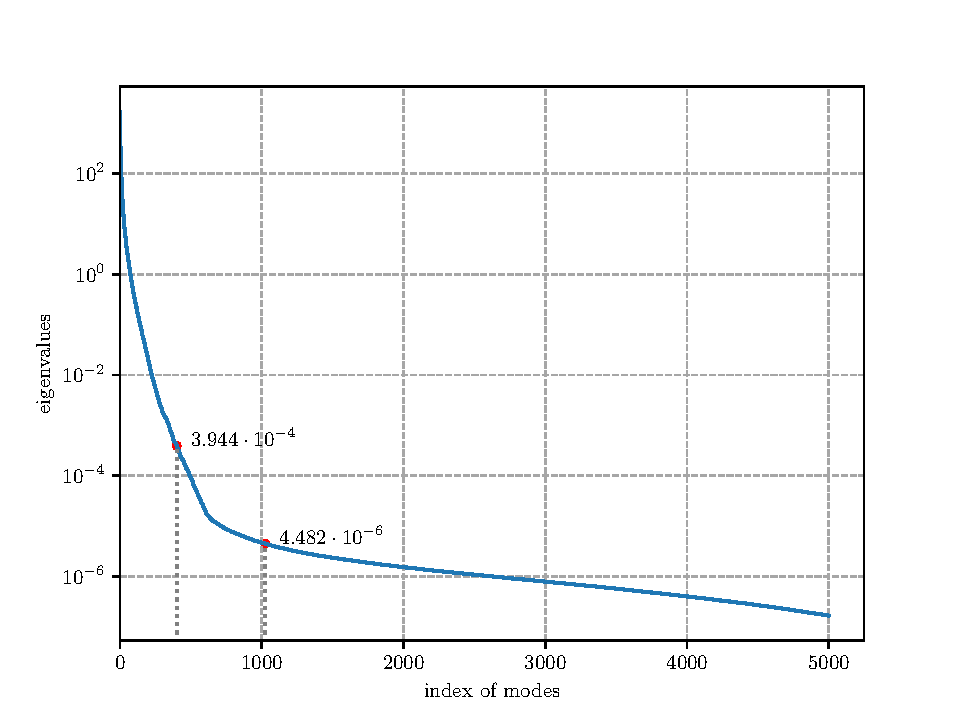
\includegraphics[width=\textwidth]{figs/eigvals_sw.pdf}
		\caption{shallow-water model}
	\end{subfigure}
	\begin{subfigure}{.4\textwidth}
		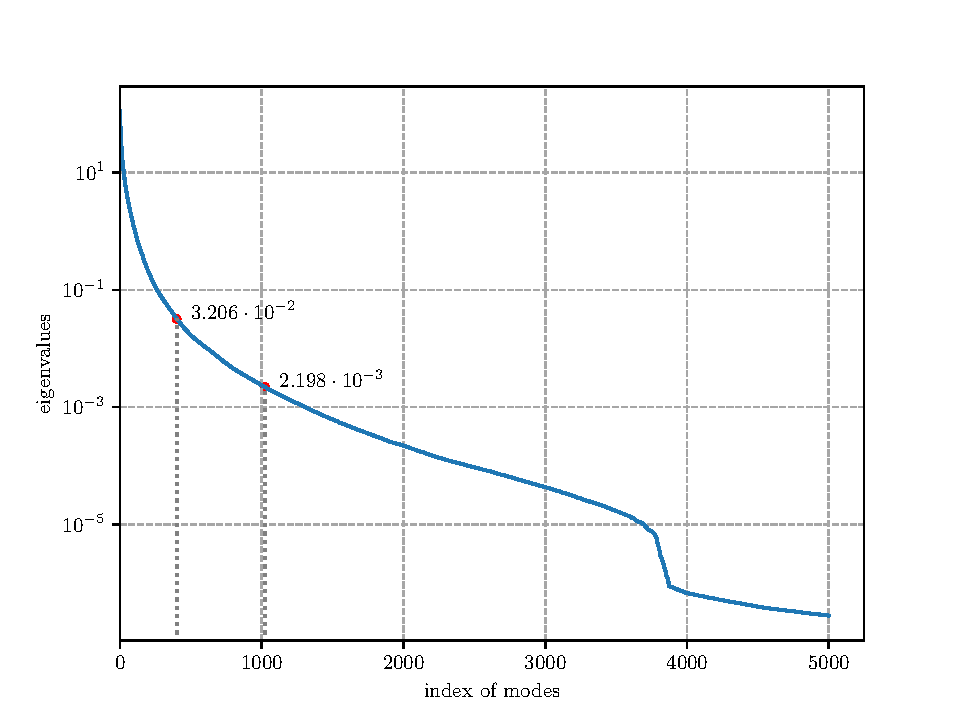
\includegraphics[width=\textwidth]{figs/eigvals_era5.pdf}
		\caption{ERA5 data}
	\end{subfigure}
	\caption{Distributions of the 5000 largest eigenvalues of the covariance matrix. The 400-th and the 1024-th eigenvalues are marked on the graph.}
	\label{fig:eigvals}
\end{figure}

For each method, we have recorded the reconstruction error on the training dataset and subsequently evaluated its generalization ability on a separate testing dataset. We adapt the following averaged reconstruction error
\[L_{\mathrm{rec}}=\frac1N\sum_{k=1}^N\weightedloss(\bm x_k,\mD\circ\mE(\bm x_k))\]
between the system states and the recovered states, where $k$ refers to the index of each snapshot and $N$ is the total amount. The reconstruction errors for both the training and testing processes are summarized in Figure \ref{fig:comp_eff}, where the numbers of latent dimensions are appended to the method names.

PCA-400 and PCA-1024 uses 400 and 1024 dominant modes, respectively. The lower training and testing errors with PCA-1024, as compared to PCA-400, signify the advantage of including more modes in reconstructing the system state, which is, however, at the cost of increased complexity and computational burden. Additionally, in spite of the low reconstruction errors on the training dataset, the testing errors are almost the same as those of AEflow and INR, which implies the PCA model tends to overfit.

When comparing to AEflow, it's important to note that the method of AEflow uses 1024 dimensions in its latent space. Even with a higher latent dimension, the AEflow method has shown relatively larger reconstruction errors in both training and testing stages, indicating its inefficiency in capturing and restoring the physical features when the latent dimensionality is limited. Contrastingly, our ROM implemented via INR utilises a lower-dimensional latent space with only 400 dimensions, which is less than half of that in AEflow and less than the number of modes used in PCA-1024. Despite this reduction in complexity, INR achieved competitive performance for the shallow-water model and even better performance for the ERA5 data than the other methods.

Upon observing the compelling performance of the encoder-decoder mappings implemented via INR, it becomes clear that our choice of employing INR as the ROM for the LA framework is well-justified. INR does not compromise the accuracy of state reconstruction and achieves competitive performance against the larger dimensional PCA-1024 and AEflow models. This not only speaks to the efficiency of INR in capturing the physical features but also points to its potential in managing the computational resources better, which means it is well suited for real-world data assimilation tasks where computational cost is a crucial factor.
\begin{figure}
	\centering
	\begin{subfigure}{.4\textwidth}
		\begin{adjustbox}{width=\textwidth}
			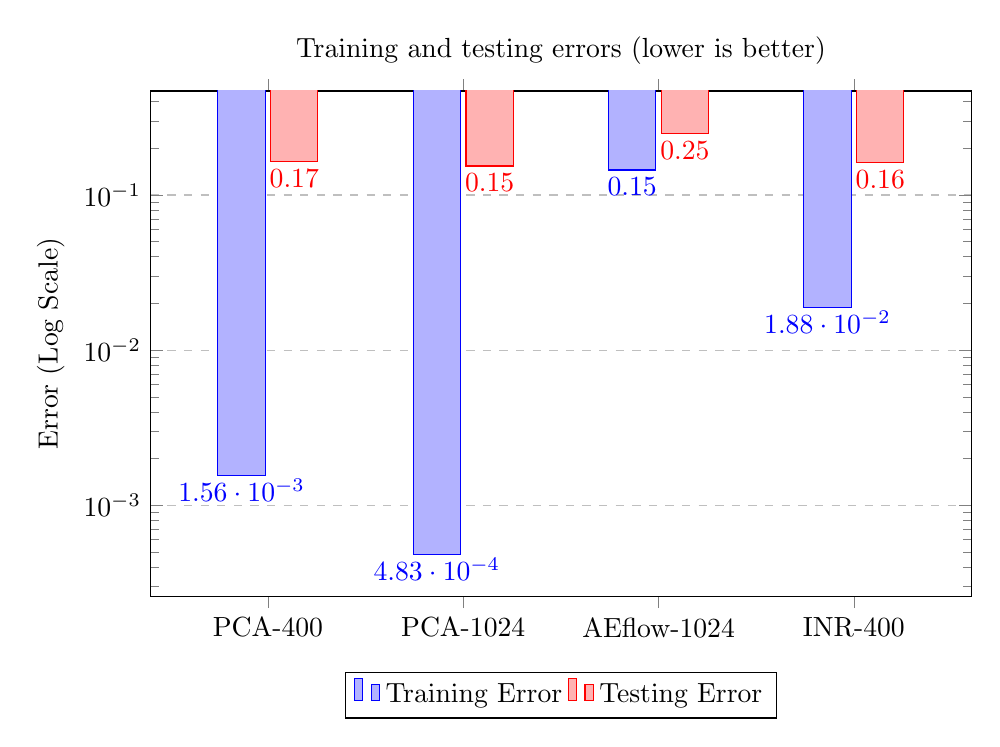
\begin{tikzpicture}
	\begin{axis}[
			title={Training and testing errors (lower is better)},
			ybar,
			ylabel={Error (Log Scale)},
			symbolic x coords={PCA-400, PCA-1024, AEflow-1024, INR-400},
			xtick=data,
			nodes near coords,
			nodes near coords align={vertical},
			every node near coord/.append style={yshift=-3ex},  % Shift the y coordinate labels up
			point meta=rawy,
			width=12cm,
			height=8cm,
			bar width=0.6cm,  % Increase the width of the bars
			enlarge x limits=0.2,
			ymode=log,  % Change Y-axis to log scale
			legend style={at={(0.5,-0.15)},
					anchor=north,legend columns=-1},
			ymajorgrids=true,
			grid style=dashed
		]
		\addplot coordinates {(PCA-400,1.56e-3) (PCA-1024,4.83e-4) (AEflow-1024,0.145) (INR-400,1.88e-2)};
		\addplot coordinates {(PCA-400,0.165) (PCA-1024,0.154) (AEflow-1024,0.251) (INR-400,0.162)};
		\legend{Training Error, Testing Error}
	\end{axis}
\end{tikzpicture}
		\end{adjustbox}
		\caption{shallow-water model}
	\end{subfigure}
	\begin{subfigure}{.4\textwidth}
		\begin{adjustbox}{width=\textwidth}
			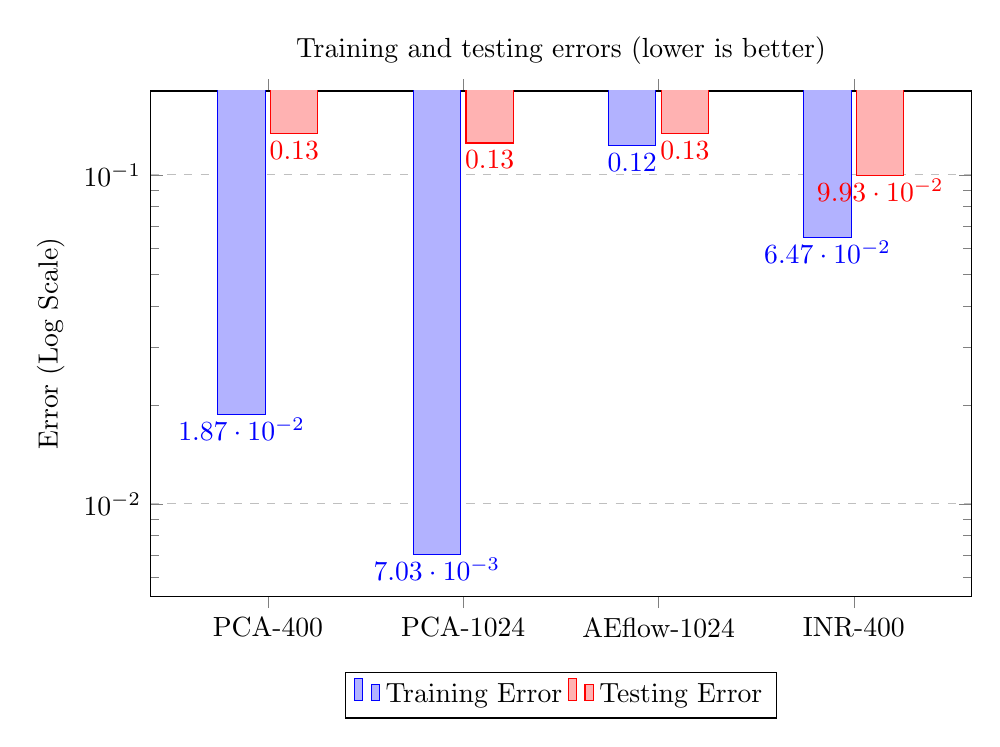
\begin{tikzpicture}
	\begin{axis}[
			title={Training and testing errors (lower is better)},
			ybar,
			ylabel={Error (Log Scale)},
			symbolic x coords={PCA-400, PCA-1024, AEflow-1024, INR-400},
			xtick=data,
			nodes near coords,
			nodes near coords align={vertical},
			every node near coord/.append style={yshift=-3ex},  % Shift the y coordinate labels up
			point meta=rawy,
			width=12cm,
			height=8cm,
			bar width=0.6cm,  % Increase the width of the bars
			enlarge x limits=0.2,
			ymode=log,  % Change Y-axis to log scale
			legend style={at={(0.5,-0.15)},
					anchor=north,legend columns=-1},
			ymajorgrids=true,
			grid style=dashed
		]
		\addplot coordinates {(PCA-400,1.87e-2) (PCA-1024,7.03e-3) (AEflow-1024,0.123) (INR-400,6.47e-2)};
		\addplot coordinates {(PCA-400,0.134) (PCA-1024,0.125) (AEflow-1024,0.134) (INR-400,9.93e-2)};
		\legend{Training Error, Testing Error}
	\end{axis}
\end{tikzpicture}
		\end{adjustbox}
		\caption{ERA5 data}
	\end{subfigure}
	\caption{Comparison of different ROMs}
	\label{fig:comp_eff}
\end{figure}

\subsubsection{embedding the physical dynamics}
Embedding a spatio-temporal dynamical system into a latent space involves not only an accurate encoding of the snapshot at each time step, but also the discovery of the latent dynamics, which is even more crucial since the latent repreasentations will be fed into a LA framework. To evaluate the consistency as well as the stability of the surrogate models for latent dynamics, the multi-step prediction error
\[L_{\mathrm{pred}}^{(s)}=\frac1N\sum_{k=1}^N\weightedloss(\bm x_{k+s},\mD\circ\mG^s\circ\mE(\bm x_k))\]
used for training is employed, where $k$ is the time index for the state $\bm x$ and $s$ indicates the number of predicting steps. The encoder-decoder mappings $\mE$ and $\mD$ are trained together with the surrogate model $\mG$ for the latent dynamics in the training process for all of the DL-based methods. The increment of the prediction error with respect to the number of predicting steps $s$ is recorded in Figure \ref{fig:comp-multi-step}.
\begin{figure}
	\centering
	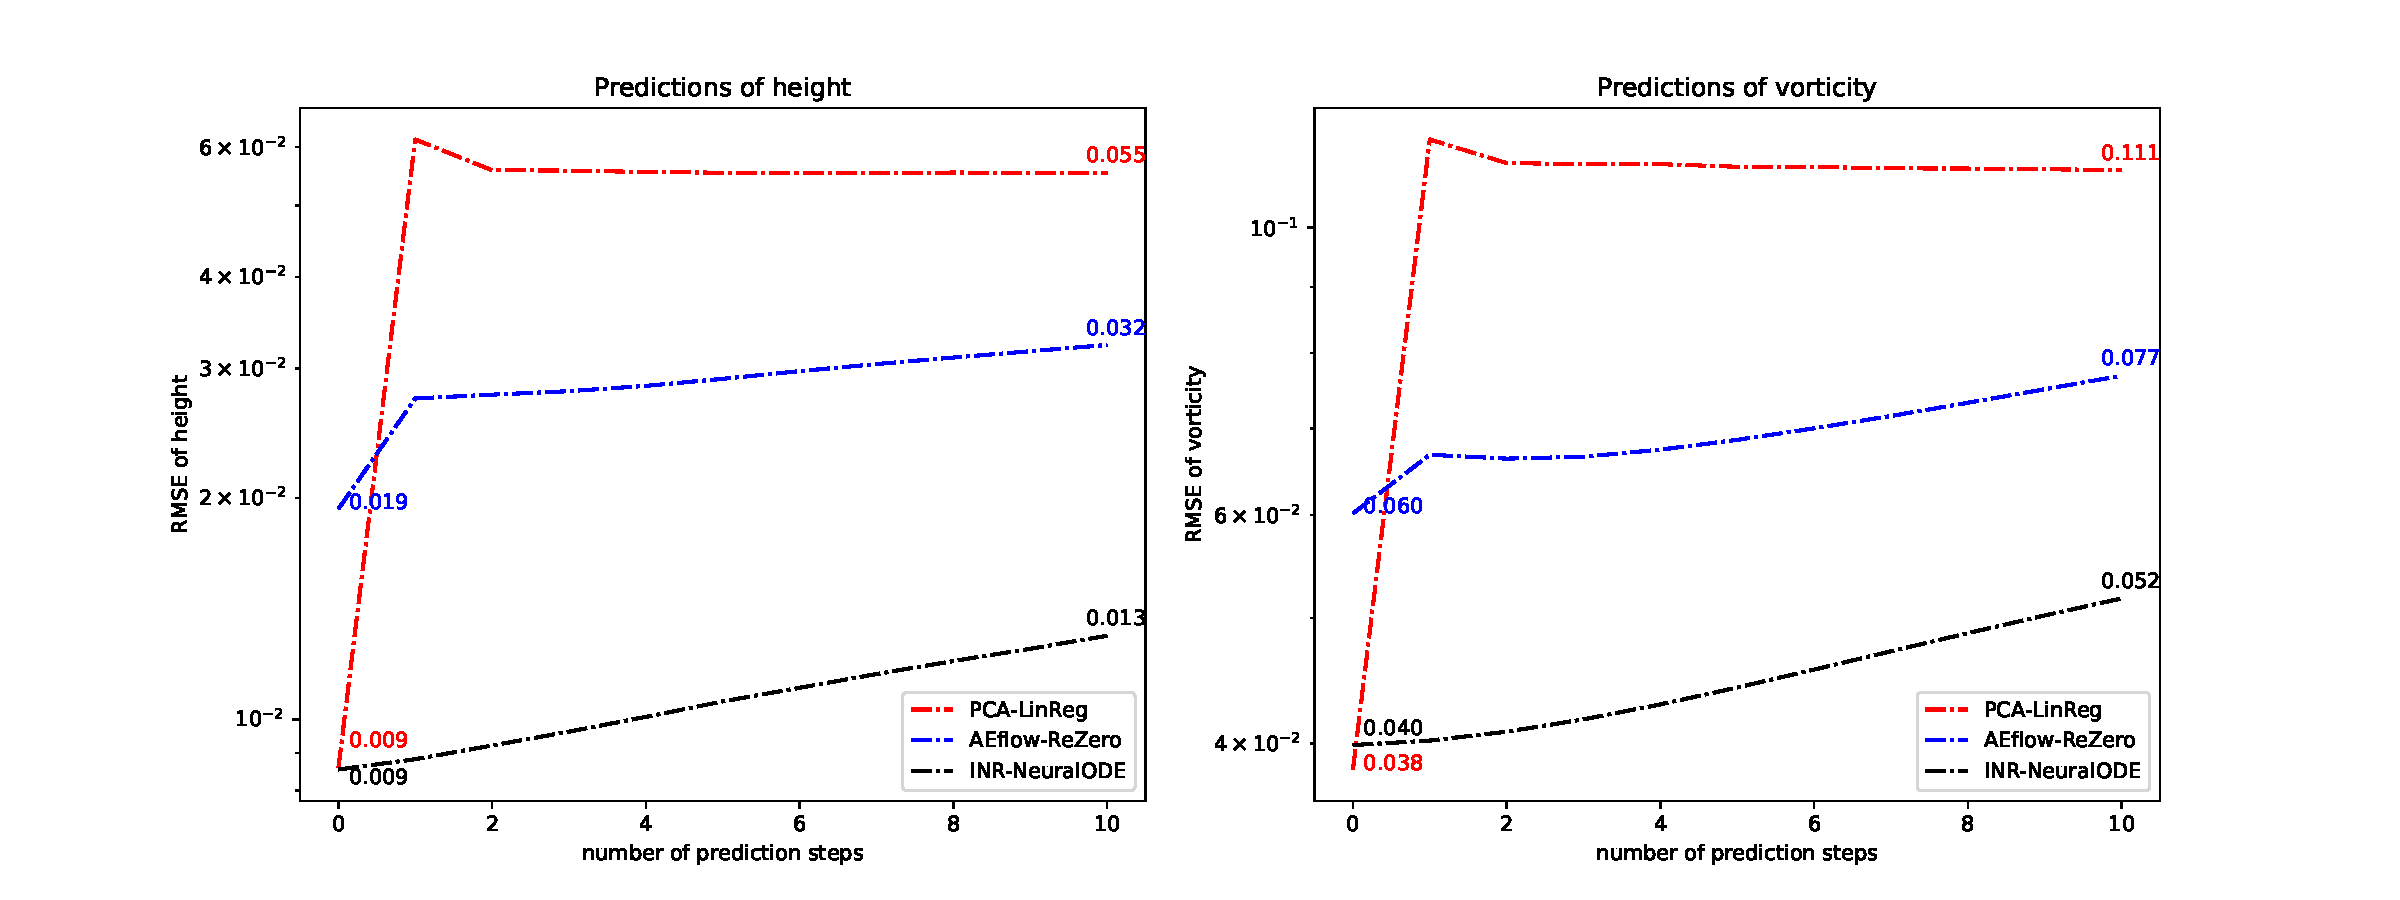
\includegraphics[width=.9\textwidth]{figs/dyn_rmse_comparison.pdf}
	\caption{Comparison of multi-step prediction error for different methods on the testing dataset}
	\label{fig:comp-multi-step}
\end{figure}
\subsubsection{compatibility (not finished yet)}
Intuitively, good performances of DA algorithms rely on the quality of the forward integrator as well as the observation operator, but an accurate surrogate model does not necessarily lead to better results since the model noise is intractable in the LA framework, and the non-linear behavior may be incompatible with the assimilation algorithm. Consequently, we check the compatibility of our proposed methods when combined with existing assimilation algorithms within the LA framework.

We choose several variants of the Kalman filter method for testing, and we would like to emphasize that similar experiments can be done with other assimilation algorithms even including the variational methods. Full algorithms for the asociated Kalman filter methods (EnKF, SEnKF, DEnKF, EnSRKF, ETKF, ETKF-Q) that involve in our experiments are all exhibited in Appendix \ref{tab:kalman_filter_methods}.

First, we fix the observation operator as a random sampling on the grid $128\times64\times2$ with the number of the observed grids $n_{\mathrm{obs}}\in\{1024,2048,4096\}$. The observation noise $\sigma^o$ is set as $0.001$, and the model noise $\sigma^m$ is tuned empirically. The initial condition is set as a perturbation of the ground truth with a Gaussian noise $\sigma^b=0.1$. See Table \ref{tab:aeflow_comparison} and Table \ref{tab:yin2023_comparison} for full results of AEflow-ReZero and INR-NeuralODE, respectively.
\begin{table}[h]
	\centering
	\caption{Comparison of performance metrics for different filters for AEflow-ReZero model.}
	\label{tab:aeflow_comparison}
	\begin{tabular}{c c c c c c c c}
		\hline
		mod\_sigma & $n_{\textrm{obs}}$ & EnKF   & SEnKF  & DEnKF  & EnSRKF & ETKF   & ETKF-Q             \\
		\hline
		1.0        & 1024               & 0.2542 & 0.2734 & 0.2764 & 0.2848 & 0.3351 & 0.1936             \\
		0.5        & 1024               & 0.2468 & 0.2294 & 0.2745 & 0.2626 & 0.2462 & 0.1914             \\
		0.2        & 1024               & 0.2559 & 0.2247 & 0.2255 & 0.2424 & 0.2163 & \underline{0.1766} \\
		0.1        & 1024               & 0.2255 & 0.2283 & 0.2084 & 0.1955 & 0.2123 & 0.2082             \\
		0.05       & 1024               & 0.2490 & 0.2391 & 0.2159 & 0.2067 & 0.2043 & 0.2968             \\
		0.02       & 1024               & 0.2759 & 0.2784 & 0.2698 & 0.2565 & 0.2493 & 0.3906             \\
		0.01       & 1024               & 0.3314 & 0.3746 & 0.3073 & 0.3478 & 0.3114 & 0.4379             \\
		\hline
		1.0        & 2048               & 0.2180 & 0.2159 & 0.2346 & 0.2236 & 0.2281 & \underline{0.1731} \\
		0.5        & 2048               & 0.2085 & 0.1958 & 0.2036 & 0.2003 & 0.1960 & 0.1837             \\
		0.2        & 2048               & 0.2028 & 0.2117 & 0.2023 & 0.2111 & 0.2035 & 0.1978             \\
		0.1        & 2048               & 0.2107 & 0.1997 & 0.2127 & 0.2448 & 0.2129 & 0.1985             \\
		0.05       & 2048               & 0.2338 & 0.2346 & 0.2092 & 0.2396 & 0.2658 & 0.2870             \\
		0.02       & 2048               & 0.2543 & 0.2752 & 0.2369 & 0.2500 & 0.2503 & 0.4051             \\
		0.01       & 2048               & 0.3246 & 0.3513 & 0.2992 & 0.3331 & 0.3156 & 0.4359             \\
		\hline
		1.0        & 4096               & 0.1953 & 0.2105 & 0.2051 & 0.1955 & 0.1963 & \underline{0.1746} \\
		0.5        & 4096               & 0.2035 & 0.1910 & 0.1911 & 0.2019 & 0.2033 & 0.1948             \\
		0.2        & 4096               & 0.1881 & 0.1947 & 0.1941 & 0.1889 & 0.1883 & 0.1905             \\
		0.1        & 4096               & 0.2077 & 0.2025 & 0.1868 & 0.1977 & 0.1966 & 0.2018             \\
		0.05       & 4096               & 0.2138 & 0.2104 & 0.2132 & 0.2004 & 0.2044 & 0.2766             \\
		0.02       & 4096               & 0.2459 & 0.2760 & 0.2277 & 0.2359 & 0.2445 & 0.4026             \\
		0.01       & 4096               & 0.3192 & 0.3583 & 0.2978 & 0.3190 & 0.3141 & 0.4393             \\
		\hline
	\end{tabular}
\end{table}
\begin{table}[h]
	\centering
	\caption{Comparison of performance metrics for different filters for INR-NeuralODE (ours).}
	\label{tab:yin2023_comparison}
	\begin{tabular}{c c c c c c c c}
		\hline
		mod\_sigma & $n_{\textrm{obs}}$ & EnKF   & SEnKF              & DEnKF  & EnSRKF             & ETKF    & ETKF-Q \\
		\hline
		0.1        & 1024               & 0.0619 & 0.0606             & 0.0645 & 0.0585             & nan     & 0.1164 \\
		0.05       & 1024               & 0.0708 & \underline{0.0575} & 0.0598 & 0.0628             & 0.0642  & 0.1290 \\
		0.02       & 1024               & 0.0590 & 0.0598             & 0.0681 & 0.0600             & 0.0615  & 0.1259 \\
		0.01       & 1024               & 0.0578 & 0.0587             & 0.0638 & 0.0581             & 0.0606  & 0.1129 \\
		0.005      & 1024               & 0.0645 & 0.0808             & 0.0686 & 0.0629             & 0.0633  & 0.1098 \\
		0.002      & 1024               & 0.1342 & 0.4105             & 0.0873 & 0.1490             & 0.1147  & 0.1436 \\
		0.001      & 1024               & 4.3256 & 1.5767             & 5.8916 & 2.9570             & 29.9085 & 0.4060 \\
		\hline
		0.1        & 2048               & 0.0454 & 0.0465             & 0.0498 & 0.0454             & nan     & 0.1252 \\
		0.05       & 2048               & 0.0442 & 0.0440             & 0.0466 & 0.0439             & 0.0445  & 0.1108 \\
		0.02       & 2048               & 0.0443 & \underline{0.0437} & 0.0463 & 0.0445             & 0.0443  & 0.1156 \\
		0.01       & 2048               & 0.0459 & 0.0449             & 0.0466 & 0.0445             & 0.0448  & 0.1275 \\
		0.005      & 2048               & 0.0518 & 0.0544             & 0.0496 & 0.0505             & 0.0501  & 0.1141 \\
		0.002      & 2048               & 0.0656 & 0.0802             & 0.0623 & 0.0751             & 0.0765  & 0.1337 \\
		0.001      & 2048               & 0.3156 & 1.0958             & 0.1431 & 0.2924             & 0.1659  & 0.1936 \\
		\hline
		0.1        & 4096               & 0.0412 & 0.0414             & 0.0433 & 0.0418             & nan     & 0.1413 \\
		0.05       & 4096               & 0.0411 & 0.0405             & 0.0420 & \underline{0.0400} & nan     & 0.1231 \\
		0.02       & 4096               & 0.0417 & 0.0420             & 0.0438 & 0.0412             & 0.0413  & 0.1145 \\
		0.01       & 4096               & 0.0416 & 0.0421             & 0.0424 & 0.0417             & 0.0416  & 0.1144 \\
		0.005      & 4096               & 0.0448 & 0.0530             & 0.0482 & 0.0467             & 0.0468  & 0.1074 \\
		0.002      & 4096               & 0.0694 & 0.1119             & 0.0637 & 0.0679             & 0.0731  & 0.1269 \\
		0.001      & 4096               & 0.1392 & 0.4200             & 0.1451 & 0.2540             & 0.2150  & 0.2179 \\
		\hline
	\end{tabular}
\end{table}

By fixing the best configurations for the two models, we have plotted the evolution of assimilated system states along with the ground truth and the differences. See Figure \ref{fig:aeflow-rezero-ass-plot} and Figure \ref{fig:ours-ass-plot} for the evolution, and Figure \ref{fig:ass-err-comp} for the corresponding assimilation error.
\begin{figure}
	\centering
	\includegraphics[width=.8\textwidth]{figs/{sigma_x_b=0.1_sigma_z_b=0.1_mod_sigma=0.1_n_obs=1024_method=ETKF-Q_plot}.png}
	\caption{AEflow-ReZero with ETKF-Q, mod\_sigma=0.1, $n_\textrm{obs}=1024$. The first 3 rows correspond to feature 0, while the last 3 rows correspond to feature 1. For each feature, the ground truth, the assimilated field as well as the corresponding differences are displayed sequentially (the frames are recorded every $40\Delta t$).}
	\label{fig:aeflow-rezero-ass-plot}
\end{figure}
\begin{figure}
	\centering
	\includegraphics[width=.8\textwidth]{figs/{fouriernet_neuralode_sigma_x_b=0.1_sigma_z_b=0.010000000000000002_mod_sigma=0.1_n_obs=1024_method=EnKF_plot_horizontal}.pdf}
	\caption{Our model with EnKF, mod\_sigma=0.1, $n_\textrm{obs}=1024$. The first 3 rows and the last 3 rows correspond to the height and the vorticity, respectively. For each feature, the ground truth, the assimilated field as well as the corresponding differences are displayed sequentially.}
	\label{fig:ours-ass-plot}
\end{figure}
\begin{figure}
	\centering
	\includegraphics[width=.4\textwidth]{figs/{sigma_x_b=0.1_sigma_z_b=0.1_mod_sigma=0.1_n_obs=1024_method=ETKF-Q_rmse}.png}
	\includegraphics[width=.4\textwidth]{figs/{sigma_x_b=0.1_sigma_z_b=0.1_mod_sigma=0.05_n_obs=1024_method=SEnKF_rmse}.png}
	\caption{Assimilation error (left: AEflow-ReZero with ETKF-Q, mod\_sigma=0.1, $n_\textrm{obs}=1024$; right: INR-NeuralODE (ours) with SEnKF, mod\_sigma=0.05, $n_\textrm{obs}=1024$)}
	\label{fig:ass-err-comp}
\end{figure}
% \subsubsection{结果分析}
% 相较于Encoder-Decoder模型(AEflow+ReZero),我们的模型除了前述INR自身的优点以外有如下优势:
% \begin{itemize}
% 	\item 数据重构和预测的精度高于AEflow+ReZero(约0.5到1个数量级);
% 	\item 结合传统同化方法时,同化误差随时间的变化更加平稳,同化误差更小(约0.5到1个数量级),且未出现发散的现象;
% 	\item 观察同化的结果图可知,我们的模型能够更好地保留物理场的结构信息,在长期运行中保持相对稳定.
% \end{itemize}
\section{Conclusion and future work}
In this paper, we have proposed a new latent assimilation framewark called Latent Assimilation with Implicit Neural Representations (LAINR), which offers an innovative integration of machine learning techniques and data assimilation concepts. Besides, our LAINR framework opens up new possibilities for processing and assimilating complex data systems by using the reduce-order technique. In comparison to classical reduced-order models (ROMs) and autoencoder-based models, experiments have shown that LAINR surpasses the previously proposed models in terms of not just theoretically appliability but also practical performance.

As a DL-based approach, LAINR employs an encoding model using Implicit Neural Representations (INR) to map the physical state into a lower-dimensional parameterization space. Simultaneously, a surrogate model implemented through Neural Ordinary Differential Equations (Neural ODEs) approximates the latent dynamics. These components together provide a powerful, high-capacity data assimilation framework that transcends many of the limitations of conventional approaches.
\paragraph{Non-linear embedding}
LAINR's capability for non-linear embedding introduces the possibility that the complex dynamics of physical states is transformed into a much simpler latent dynamics. This feature stands in contrast with classical linear ROMs including the PCA-LinReg method as tested in our experiments, which may inadequently represent complex system dynamics.
\paragraph{Continuous mapping}
Unlike classical linear ROMs or autoencoder-based models that treat the state field as a discrete grid of state features, LAINR considers the state field as a continuous map, and the special perspective provides a more accurate description of physical features, aiding in the learning of latent representations.
\paragraph{Flexibility of inputs}
While classical ROMs and autoencoder architectures requires fully provided input data for embedding process, LAINR is able to handle inputs from partially observed or even irregular grids, which becomes more suitable under potential hardware limitations when complete observations are not always guaranteed such as satellite or radar observations, and as a consequence, its utility scope is wider in real-world scenarios.
\paragraph{Scalability}
LAINR exhibits a clear edge in scalability over previous autoencoder-based models. Since the architecture of LAINR uses coordinates as inputs, it effortlessly accommodates increasing dimensionality and resolution, unlike classical models that encounter increased computational costs due to their reliance on a grid of features as inputs.

Experimental results have demonstrated that our LAINR framework is not only theoretically sound but also practically efficient and effective. It has also been shown that LAINR has superior performance in terms of prediction accuracy compared to previous works, which indicates that the LAINR framework is a promising alternative in the realm of data assimilation especially when no accurate forward integrator is available. Its non-linear embedding capability and continuous mapping methodology allow a more accurate depiction and interpretation of complex systems. Its flexibility in handling partial and irregular input data makes it robust for real-world applications, while its scalability makes it highly suitable for managing the burgeoning volumes of data in this era of big data.

Nonetheless, we have to stress that the full potential of LAINR has not yet been expored, and it is also important to acknowledge that areas where further research and development are needed. One such aspect is the testing of LAINR in real datasets such as the ERA5 dataset \cite{ERA5}. The performance and robustness of our LAINR framework under real-world conditions would provide further validation of its effectiveness. Additionally, more complicated observation operators need to be incorporated into the experiments since the real observations tends to be highly non-linear such as the solution of radiative-transfer models. Moreover, future work should explore the design of more advanced architectures for INR as well. As the model error is tuned empirically at present, new structures considering the embedding error and the prediction error are likely to provide a more comprehensive and accurate model.

In conclusion, LAINR brings a heightened level of intricacy, scalability, and flexibility to the handling of complex systems. As we continue to traverse the era of big data and complex systems, trailblazing frameworks like LAINR will be indispensable in augmenting our predictive capabilities and understanding of complex systems. With its full potential yet to be explored, LAINR promises to catalyze a paradigm shift in our interaction with and comprehension of complex systems.
\bibliographystyle{plain} % We choose the "plain" reference style
\bibliography{LAINR} % Entries are in the refs.bib file
\appendix
\section{Mathematical preliminaries}
\begin{Prop}\label{prop:pod_optimality}
	Given $\{x_k\}_{k=1}^K\subseteq\mR^n$, the matrix consists of the first $m$ ($m<n$) left singular vectors of the matrix $X=(x_1,\cdots,x_K)\in\mR^{n\times K}$ solves the following minimization problem:
	\[\min_A\sum_{k=1}^K\left\|x_k-A^\trans A x_k\right\|^2=\min_A\left\|(I-A^\trans A)X\right\|_F^2\textrm{ subject to }AA^\trans=I_m\]
	for $A\in\mR^{m\times n}$, where $\|\cdot\|_F$ is the Frobenius norm.
\end{Prop}
\begin{proof}
	For any $A\in\mR^{m\times n}$ satisfying $AA^\trans=I_m$ we have
	\begin{align*}
		\sum_{k=1}^K\left\|x_k-A^\trans A x_k\right\|^2 & =\sum_{k=1}^K\left\|x_k\right\|^2-2x_k^\trans A^\trans Ax_k+\left\|A^\trans A x_k\right\|^2             \\
		                                                & =\sum_{k=1}^K\left\|x_k\right\|^2-2x_k^\trans A^\trans Ax_k+x_k^\trans A^\trans AA^\trans A x_k         \\
		                                                & =\sum_{k=1}^K\left\|x_k\right\|^2-x_k^\trans A^\trans Ax_k=\sum_{k=1}^K\left\|x_k\right\|^2-\|Ax_k\|^2.
	\end{align*}
	Hence the minimization problem is equivalent to the maximization problem
	\[\max_A\sum_{k=1}^K\|Ax_k\|^2=\max_A\|AX\|_F^2\textrm{ subject to }AA^\trans=I_m.\]
	Take the singular-value decomposition (SVD) for the matrix $X$ as $X=U\Sigma V^\trans$, where $U\in\mR^{n\times n}$ and $V\in\mR^{K\times K}$ are orthogonal matrices and $\Sigma=\diag(\sigma_1,\cdots,\sigma_s)$ with $s=\min(n,K)$ and $\sigma_1\geq\cdots\geq\sigma_s\geq0$. It follows that
	\[\|AX\|_F^2=\tr\left(AX(AX)^\trans\right)=\tr\left(AU\Sigma V^\trans V\Sigma^\trans UA^\trans\right)=\tr\left(AU\Sigma\Sigma^\trans UA^\trans\right)=\sum_{l=1}^s\sigma_l^2\|Au_l\|^2,\]
	where $u_l$ is the $l$-th column of $U$, which is also the left singular vector corresponding to the singular value $\sigma_l$. Note that
	\[\sum_{l=1}^s\|Au_l\|^2\le\|AU\|_F^2=\tr(AUU^\trans A^\trans)=\tr(AA^\trans)=\|A\|_F^2=m.\]
	Meanwhile, let $B\in\mR^{(n-m)\times n}$ such that $(A^\trans, B^\trans)$ is orthogonal, then for each $l$,
	\[\|Au_l\|^2=u_l^\trans A^\trans Au_l=u_l(I_n-B^\trans B)u_l=\|u_l\|^2-\|Bu_l\|^2\le\|u_l\|^2=1.\]
	Therefore,
	\begin{align*}
		\sum_{l=1}^s\sigma_l\|Au_l\|^2 & =\sum_{l=1}^m\sigma_l^2+\sum_{l=1}^m\sigma_l^2\left(\|Au_l\|^2-1\right)+\sum_{l=m+1}^s\sigma_l^2\|Au_l\|^2   \\
		                               & \le\sum_{l=1}^m\sigma_l^2+\sigma_m^2\sum_{l=1}^m\left(\|Au_l\|^2-1\right)+\sigma_m^2\sum_{l=m+1}^s\|Au_l\|^2 \\
		                               & =\sum_{l=1}^m\sigma_l^2+\sigma_m^2\left(\sum_{l=1}^s\|Au_l\|^2-m\right)\le\sum_{l=1}^m\sigma_l^2.
	\end{align*}
	Additionally, it is clear that all the equalities hold if $A=(u_1,\cdots,u_m)^\trans$.
\end{proof}
\section{Detailed configurations for the experiments}\label{sec:exp_configs}
Most of the configurations are borrowed from \cite{Galewsky-2004} and \cite{Nicholas2015QGsetting} for shallow-water equations and the QG-model, respectively. We restate them here together with dataset configurations for completeness. Note that all the fixed parameters are of SI units (the International System of Units) and thus omitted for simplicity.
\subsection{shallow-water equations}
The spherical shallow-water equations on the 2D sphere read
\begin{align*}
	\frac{\md\bm u}{\md t} & =-f\bm k\times\bm u-g\nabla h+\nu\Delta\bm u, \\
	\frac{\md h}{\md t}    & =-h\nabla\cdot\bm u+\nu\Delta h,
\end{align*}
where $\bm u=(u,v)^\trans$ is the 2D velocity field tangent to the sphere surface, and $h$ is the thickness of the fluid layer, both of which are defined on a channel domain $(\lambda,\phi)\in[0,2\pi]\times[-\pi/2,\pi/2]$. The Coriolis parameter $f=2\Omega\sin\phi$ with the angular velocity $\Omega=7.292\times10^{-5}$ and the gravity $g=9.80616$ are fixed in consistency with the real earth surface. The viscosity coefficient $\nu=\frac{10^5\times3600^2}{a^2\times32^2}\approx3.1\times10^{-7}$ with the earth radius $a=6.37122\times10^6$ is chosen to be small enough to avoid damping the physical features. The initial conditions for $\bm u$ are given by
\[
	v|_{t=0}=0,\quad u|_{t=0}=
	\begin{cases}
		\frac{u_m}{e_n}\exp\left(\frac1{(\phi-\phi_0)(\phi-\phi_1)}\right), & \phi_0<|\phi|<\phi_1, \\
		0                                                                   & \textrm{otherwise},
	\end{cases}
\]
which is slightly modified from \cite{Galewsky-2004} to create symmetric fields, where $\phi_0=\pi/7$ and $\phi_1=\pi/2-\phi_0$ gives the boundary of the jet. $e_n=\exp(-4/(\phi_1-\phi_0)^2)$ is the normalizer so that the maximal zonal wind $u_m$ lies at the jet's mid-point. The thickness $h$ is initialized as a balanced height field, which is obtained by integrating the balance equation
\[gh(\phi)=gh_0-\int^\phi au(\phi')\left(f+a^{-1}u(\phi')\tan\phi'\right)\md \phi'.\]
The constant $h_0$ is chosen so that the global mean of $h$ is $10^4$. The balanced field is then perturbed by adding a localized bump
\[h'(\lambda,\phi)=\hat h\exp(-(\lambda/\alpha)^2-((\phi_2-\phi)/\beta)^2)\cos\phi,\]
where $\hat h=120$, $\alpha=1/3$, $\beta=1/15$, and $\phi_2=\pi/4$.

The datasets for both training and testing are generated via the Dedalus project \cite{dedalus} based on Python language within a spectral framework. The maximum velocity $u_m$ is chosen from $\{60,61,\cdots,80\}$ to generate distinct 21 trajectories for separation of training and testing. Each trajectory has been recorded from 300 hours to 700 hours with 1-hour interval to capture rich physical features, and the spatial resolution is set as $128\times64$. The vorticity $w=\nabla\times\bm u$ and the thickness $h$ are the two features for network training and assimilation.
% \subsection{quasi-geostrophic (QG) equations}
% We follow the settings of a nondimensional version of the two-layered quasi-geostrophic equation on a zonally periodic channel described in \cite{Nicholas2015QGsetting,Chattopadhyay2021DeepST}
% \[\frac{\partial q_k}{\partial t}+J(\psi_k,q_k)=-\tau_d^{-1}(-1)^k(\psi_1-\psi_2-\psi_R)-\tau_f^{-1}\delta_{k2}\nabla^2\psi_k-\nu\nabla^8q_k,\,k=1,2,\]
% where
% \[q_k=\nabla^2\psi_k+(-1)^k(\psi_1-\psi_2)+\beta y\]
% is the potential vorticity for the upper ($k=1$) and lower ($k=2$) layers with the corresponding streamfunction $\psi_k$. $J$ denotes the Jacobian operator and $\delta$ is the Kronecker function to impose frictional dissipation only on the lower layer. $\tau_d=100$ and $\tau_f=15$ represent the Newtonian relaxation time scale and the Rayleigh friction time scale, respectively. $\beta=0.196$ is the Rossby parameter, and $\nu=0.01$ is the hyperdiffusion coefficient.

% To start the simulation, a baroclinically unstable jet is created in the center of the domain by setting the radiative equilibrium temperature $(\psi_1-\psi_2)$ profile to a hyperbolic secant function centered at $y=0$. The low-layer $\psi_2$ is initialized as identically zero in radiative equilibrium so that the zonal flow in the upper layer
% \[u_1(y)=-\frac{\partial\psi_1}{\partial y}=-\frac{\partial\psi_R}{\partial y}=\sech^2(y/\sigma)\]w
% with the width of the jet $\sigma=3.5$ (scaled). The domain size is set as $(L_x,L_y)=(46,23)$ with the grid size $128\times192$.
% The work of \cite{Nabizadeh2019QGcode} has provided a detailed Matlab code for data generation. The initial fields are perturbed with small-scale noise to generate different trajectories. Each trajectory consist of 10000[\textcolor{red}{need check}] snapshots with $\Delta t=0.2$ model day, which corresponding to 1 hour in reality. Note that the generated trajectories are truncated and then downsampled to a grid size of $128\times64$ to avoid the boundary effects as mentioned in \cite{Chattopadhyay2021DeepST}.
\section{Algorithms for associated Kalman filter methods}\label{tab:kalman_filter_methods}
\subsection{EnKF}
The basic Ensenble Kalman Filter (EnKF)
\subsubsection{Forecast step}
\begin{itemize}
	\item Forward propagation:
	      $$
		      x_k^{b,j}=\mathcal{M}_k(x_{k-1}^{a,j})+\varepsilon_k^{M,j},\quad \varepsilon_k^{M,j}\sim\mathcal{N}(0,\Sigma_k^M);
	      $$
	      perturbed propagation

\end{itemize}
\subsubsection{Analysis step}
\begin{itemize}
	\item Obtain the ensemble mean and anomaly matrix from the ensembles:
	      \begin{align*}
		      x_k^b & = \frac1N\sum_{j=1}^Nx_k^{b,j},                                           \\
		      X_k^b & = \frac1{\sqrt{N-1}}(x_k^{b,j} - x_k^b)_{j=1}^N\in\mathbb{R}^{n\times N}, \\
		      P_k^b & = X_k^bX_k^{b\trans}
	      \end{align*}
	\item Obtain the perturbed observation vectors:
	      $$
		      z_k^{o,j} = y_k^o + \varepsilon_k^{o,j},\quad\varepsilon_k^{o,j}\sim\mathcal{N}(0,\Sigma_k^o);
	      $$
	\item Innovation vectors
	      $$
		      d_k^j = z_k^{o,j} - \mathcal{H}_k(x_k^{b,j});
	      $$
	\item Evaluate the Kalman gain matrix
	      \begin{align*}
		      K_k & = P_k^bH_k^\trans (H_kP_k^bH_k^\trans +\Sigma_k^o)^{-1}                           \\
		          & = X_k^bX_k^{b\trans}H_k^\trans (H_kX_k^bX_k^{b\trans}H_k^\trans +\Sigma_k^o)^{-1} \\
		          & = P_{xz}(P_{zz}+\Sigma_k^o)^{-1},
	      \end{align*}
	      where
	      $$
		      P_{xz} = X_k^b(H_kX_k^b)^\trans ,\quad P_{zz} = (H_kX_k^b)(H_kX_k^b)^\trans .
	      $$
	\item Update the analyzed ensembles:
	      $$
		      x_k^{a,j}=x_k^{b,j}+K_kd_k^j.
	      $$
\end{itemize}
\subsection{SEnKF}
Stochastic EnKF (Algorithm 6.3 in \cite{Bocquet2016})
\subsubsection{Forecast step}
\begin{itemize}
	\item Forward propagation:
	      $$
		      x_k^{b,j}=\mathcal{M}_k(x_{k-1}^{a,j})+\varepsilon_k^{M,j},\quad \varepsilon_k^{M,j}\sim\mathcal{N}(0,\Sigma_k^M);
	      $$
	      perturbed propagation
\end{itemize}


\subsubsection{Analysis step}
\begin{itemize}
	\item Obtain the ensemble mean and anomaly matrix from the ensembles:
	      \begin{align*}
		      x_k^b & = \frac1N\sum_{j=1}^Nx_k^{b,j},                                           \\
		      X_k^b & = \frac1{\sqrt{N-1}}(x_k^{b,j} - x_k^b)_{j=1}^N\in\mathbb{R}^{n\times N}, \\
		      P_k^b & = X_k^bX_k^{b\trans}
	      \end{align*}
	\item Obtain the perturbed observation vectors:
	      $$
		      z_k^{o,j} = y_k^o + \varepsilon_k^{o,j},\quad\varepsilon_k^{o,j}\sim\mathcal{N}(0,\Sigma_k^o);
	      $$
	\item Compute the ensemble means and the normalized anomalies for the perturbed background estimates for the observations:
	      \begin{align*}
		      y_k^{p,j} & = \mathcal{H}_k(x_k^{b,j}) - \varepsilon_k^{o,j}                          \\
		      y_k^p     & = \frac1N\sum_{j=1}^Ny_k^{p,j},                                           \\
		      Y_k^p     & = \frac1{\sqrt{N-1}}(y_k^{p,j} - y_k^p)_{j=1}^N\in\mathbb{R}^{n\times N}.
	      \end{align*}
	\item Kalman gain matrix
	      $$
		      K_k=X_k^bY_k^{pT}(Y_k^pY_k^{pT})^{-1}
	      $$
	\item Update the analyzed ensembles:
	      $$
		      x_k^{a,j}=x_k^{b,j}+K_k(z_k^{o,j}-\mathcal{H}_k(x_k^{b,j})).
	      $$
\end{itemize}
\subsection{DEnKF}
EnSRKF (See (6.25) in \cite{Bocquet2016})
\subsubsection{Forecast step}
\begin{itemize}
	\item Forward propagation:
	      $$
		      x_k^{b,j}=\mathcal{M}_k(x_{k-1}^{a,j})+\varepsilon_k^{M,j},\quad \varepsilon_k^{M,j}\sim\mathcal{N}(0,\Sigma_k^M);
	      $$
	      perturbed propagation
\end{itemize}

\subsubsection{Analysis step}
\begin{itemize}
	\item Obtain the ensemble mean and anomaly matrix from the ensembles:
	      \begin{align*}
		      x_k^b & = \frac1N\sum_{j=1}^Nx_k^{b,j},                                           \\
		      X_k^b & = \frac1{\sqrt{N-1}}(x_k^{b,j} - x_k^b)_{j=1}^N\in\mathbb{R}^{n\times N}, \\
		      P_k^b & = X_k^bX_k^{b\trans}
	      \end{align*}
	\item Innovation vectors
	      $$
		      d_k = y_k^o - \mathcal{H}_k(x_k^b);
	      $$
	\item Kalman gain matrix
	      \begin{align*}
		      K_k & = P_k^bH_k^\trans (H_kP_k^bH_k^\trans +\Sigma_k^o)^{-1}                           \\
		          & = X_k^bX_k^{b\trans}H_k^\trans (H_kX_k^bX_k^{b\trans}H_k^\trans +\Sigma_k^o)^{-1} \\
		          & = P_{xz}(P_{zz}+\Sigma_k^o)^{-1},
	      \end{align*}
	\item Assimilate the forecast state estimate with the observation
	      $$
		      x_k^a = x_k^b + K_k(y_k^o - \mathcal{H}_k(x_k^b))
	      $$
	\item Compute the analyzed anomalies
	      $$
		      X_k^a = X_k-\frac12K_kH_kX_k
	      $$
	\item Compute the analyzed ensembles
	      $$
		      x_k^{a,j} = \sqrt{N-1}X_k^a[:, j] + x_k^a
	      $$
\end{itemize}
\subsection{EnSRKF}
EnSRKF (See (6.21) in \cite{Bocquet2016})

\subsubsection{Forecast step}
\begin{itemize}
	\item Forward propagation:
	      $$
		      x_k^{b,j}=\mathcal{M}_k(x_{k-1}^{a,j})+\varepsilon_k^{M,j},\quad \varepsilon_k^{M,j}\sim\mathcal{N}(0,\Sigma_k^M);
	      $$
	      perturbed propagation
\end{itemize}

\subsubsection{Analysis step}
\begin{itemize}
	\item Obtain the ensemble mean and anomaly matrix from the ensembles:
	      \begin{align*}
		      x_k^b & = \frac1N\sum_{j=1}^Nx_k^{b,j},                                           \\
		      X_k^b & = \frac1{\sqrt{N-1}}(x_k^{b,j} - x_k^b)_{j=1}^N\in\mathbb{R}^{n\times N}, \\
		      P_k^b & = X_k^bX_k^{b\trans}
	      \end{align*}
	\item Compute the ensemble means and the normalized anomalies for the observations:
	      \begin{align*}
		      y_k^{b,j} & = \mathcal{H}_k(x_k^{b,j})                                                \\
		      y_k^b     & = \frac1N\sum_{j=1}^Ny_k^{b,j},                                           \\
		      Y_k^b     & = \frac1{\sqrt{N-1}}(y_k^{b,j} - y_k^b)_{j=1}^N\in\mathbb{R}^{m\times N};
	      \end{align*}
	\item Transforming matrix
	      $$
		      T_k = (I_m+Y_k^{b\trans}(\Sigma_k^o)^{-1}Y_k^b)^{-1} = (I_m + S_k^\trans S_k)^{-1}
	      $$
	      for $S_k=(\Sigma_k^o)^{-1/2}Y_k^b$;

	\item normalized innovation vector
	      $$
		      \delta_k = (\Sigma_k^o)^{-1/2}(y_k^o-y_k^b)
	      $$
	\item Evaluate the original Kalman gain matrix
	      \begin{align*}
		      K_k & = P_k^bH_k^\trans (H_kP_k^bH_k^\trans +\Sigma_k^o)^{-1}                           \\
		          & = X_k^bX_k^{b\trans}H_k^\trans (H_kX_k^bX_k^{b\trans}H_k^\trans +\Sigma_k^o)^{-1} \\
		          & = P_{xz}(P_{zz}+\Sigma_k^o)^{-1},
	      \end{align*}
	      where
	      $$
		      P_{xz} = X_k^b(H_kX_k^b)^\trans ,\quad P_{zz} = (H_kX_k^b)(H_kX_k^b)^\trans .
	      $$
	\item Obtain the modified Kalman gain matrix
	      $$
		      \tilde K = K(I + (I + H_kP_k^bH_k^\trans (\Sigma_k^o)^{-1})^{-1/2})^{-1}
	      $$
	\item Update the analyzed ensembles
	      \begin{align*}
		      w_k^a     & = (I_m + Y_k^{b\trans}\Sigma_k^o Y_b)^{-1}Y^{b\trans}(\Sigma_k^o)^{-1}(y_k^o-y_k^b)=T_kS_k^\trans \delta_k \\
		      x_k^a     & = x_k^b + X_k^bw_k^a = x_k^b + X_k^bT_kS_k^\trans \delta_k                                                 \\
		      X_k^a     & = (I_n - \tilde{K}_kH_k)X_k^bU,\, U1=1, U\in O(N)                                                          \\
		      x_k^{a,j} & = x_k^a + \sqrt{N-1}X_k^a[:, j]
	      \end{align*}
	      OR:
	      $$
		      (x_k^{a,j})_j = x_k^b1_N^\trans  + \sqrt{N-1}X_k^a
	      $$
\end{itemize}

\subsection{ETKF}
ETKF (Algorithm 6.4 in \cite{Bocquet2016})

\subsubsection{Forecast step}
\begin{itemize}
	\item Forward propagation:
	      $$
		      x_k^{b,j}=\mathcal{M}_k(x_{k-1}^{a,j})+\varepsilon_k^{M,j},\quad \varepsilon_k^{M,j}\sim\mathcal{N}(0,\Sigma_k^M);
	      $$
	      perturbed propagation
\end{itemize}

\subsubsection{Analysis step}
\begin{itemize}
	\item Obtain the ensemble mean and anomaly matrix from the ensembles:
	      \begin{align*}
		      x_k^b & = \frac1N\sum_{j=1}^Nx_k^{b,j},                                           \\
		      X_k^b & = \frac1{\sqrt{N-1}}(x_k^{b,j} - x_k^b)_{j=1}^N\in\mathbb{R}^{n\times N}, \\
		      P_k^b & = X_k^bX_k^{b\trans}
	      \end{align*}
	\item Compute the ensemble means and the normalized anomalies for the observations:
	      \begin{align*}
		      y_k^{b,j} & = \mathcal{H}_k(x_k^{b,j})                                                \\
		      y_k^b     & = \frac1N\sum_{j=1}^Ny_k^{b,j},                                           \\
		      Y_k^b     & = \frac1{\sqrt{N-1}}(y_k^{b,j} - y_k^b)_{j=1}^N\in\mathbb{R}^{m\times N};
	      \end{align*}
	\item Transforming matrix
	      $$
		      T_k = (I_N+Y_k^{b\trans}(\Sigma_k^o)^{-1}Y_k^b)^{-1} = (I_N + S_k^\trans S_k)^{-1}
	      $$
	      for $S_k=(\Sigma_k^o)^{-1/2}Y_k^b$;

	\item normalized innovation vector
	      $$
		      \delta_k = (\Sigma_k^o)^{-1/2}(y_k^o-y_k^b)
	      $$
	\item Update the analyzed ensembles:
	      \begin{align*}
		      w_k^a     & = (I_N + Y_k^{b\trans}(\Sigma_k^o)^{-1} Y_k^b)^{-1}Y^{b\trans}(\Sigma_k^o)^{-1}(y_k^o-y_k^b)=T_kS_k^\trans \delta_k \\
		      x_k^a     & = x_k^b + X_k^bw_k^a = x_k^b + X_k^bT_kS_k^\trans \delta_k                                                          \\
		      X_k^a     & = X_k^b(I_N+Y_k^{b\trans}(\Sigma_k^o)^{-1}Y_k^b)^{-1/2}U,\, U1=1, U\in O(N)                                         \\
		      x_k^{a,j} & = x_k^a + \sqrt{N-1}X_k^a[:, j]                                                                                     \\
		                & = x_k^b + X_k^b(w_k + \sqrt{N-1}T^{1/2}U[:, j])
	      \end{align*}
	      OR:
	      $$
		      (x_k^{a,j})_j = x_k^b1_N^\trans  + X_k^b(w_k1_N^\trans +\sqrt{N-1}T_k^{1/2}U)
	      $$
\end{itemize}

\subsection{ETKF-Q}
The ETKF-Q algorithm borrowed from \cite{Peyron2021LAwithAE} (a special case of IEnKS-Q \cite{Fillion2020IEnKS}).

\subsubsection{Initialization}

Construct $U\in\mathbb{R}^{N\times(N-1)}$ such that
$$
	\begin{pmatrix}
		\frac1{\sqrt N}1_N & U
	\end{pmatrix}
$$
is orthogonal, and let
$$
	\mathscr{U}=
	\begin{pmatrix}
		\frac1N1_N & \frac{1}{\sqrt{N-1}}U
	\end{pmatrix},
$$
then
$$
	\mathscr{U}^{-1}=
	\begin{pmatrix}
		1_N & \sqrt{N-1}U
	\end{pmatrix}^\trans ,
$$

\subsubsection{Forecast step}
\begin{itemize}
	\item Forward propagation:
	      $$
		      x_k^{f,j}=\mathcal{M}_k(x_{k-1}^{a,j});
	      $$
	\item obtain the mean and deviation for $x_k^f$
	      $$
		      (x_k^f,\Delta_x^f)=(x_k^{f,j})_j\mathscr{U}
	      $$
	\item eigen decomposition (approximately):
	      $$
		      (\Delta_x^f\Delta_x^{f\trans}+\Sigma_k^M)V_k\approx V_k\Lambda_k,
	      $$
	      where $V_k\in\mathbb{R}^{n\times(N-1)}$ and $\Lambda_k\in\mathbb{R}^{(N-1)\times(N-1)}$ are the eigenvectors and eigenvalues of $\Delta_x^f\Delta_x^{f\trans}+\Sigma_k^M$;
	\item update the deviation:
	      $$\Delta_x^b=V_k\Lambda_k^{1/2}$$
	\item update the ensembles:
	      $$(x_k^{b,j})_j=(x_k^f,\Delta_x^b)\mathscr{U}^{-1}$$
\end{itemize}

\subsubsection{Analysis step}
\begin{itemize}
	\item Obtain the ensemble mean and deviation matrix from the ensembles:
	      $$
		      (x_k^b,\Delta_x^b)=(x_k^{b,j})_j\mathscr{U}
	      $$
	\item obtain the mean and deviation for background estimates of observations:
	      \begin{align*}
		      y_k^{b,j}          & =\mathcal{H}_k(x_k^{b,j}) \\
		      (y_k^b,\Delta_y^b) & =(y_k^{b,j})_j\mathscr{U}
	      \end{align*}
	\item Transforming matrix:
	      $$
		      T_k=(I_{N-1}+\Delta_y^{b\trans}(\Sigma_k^o)^{-1}\Delta_y^b)^{-1}=(I_{N-1} + S_k^\trans S_k)^{-1}
	      $$
	      for $S_k=(\Sigma_k^o)^{-1/2}\Delta_y^b$;

	\item normalized innovation vector
	      $$
		      \delta_k = (\Sigma_k^o)^{-1/2}(y_k^o-y_k^b)
	      $$
	\item Update the analyzed ensembles: (modified from ETKF)
	      \begin{align*}
		      w_k^a      & = (I_{N-1} + \Delta_y^{b\trans}\Sigma_k^o \Delta_y^b)^{-1}\Delta_y^{b\trans}(\Sigma_k^o)^{-1}(y_k^o-y_k^b)=T_kS_k^\trans \delta_k \\
		      x_k^a      & = x_k^b + \Delta_x^bw_k^a = x_k^b + \Delta_x^bT_kS_k^\trans \delta_k                                                              \\
		      \Delta_x^a & = \Delta_x^b(I_{N-1}+\Delta_y^{b\trans}(\Sigma_k^o)^{-1}\Delta_y^b)^{-1/2}                                                        \\
		      x_k^{a,j}  & = (x_k^a,\Delta_x^a)\mathscr{U}^{-1}
	      \end{align*}
\end{itemize}
\section{Implementation}
We provide the proposed LAINR framework on Github, with the following detailed explanation and psedo-codes.
\end{document}